\documentclass[/home/jesse/Analysis/FemtoAnalysis/AnalysisNotes/AnalysisNoteJBuxton.tex]{subfiles}
\begin{document}

\subsection{Residual Correlations}
\label{ResidualCorrelations}

The purpose of this analysis is study the interaction and scale of the emitting source of the primary \LamK pairs.
In order to obtain correct results, it is desirable for our particle collections to consist of primary particles.
In practice, this is impossible to achieve; many of our particles are not primary, but originate as decay products from other resonances.
Some of our \Lam hyperons decay from $\Sigma^{0}$, $\Xi^{0}$, $\Xi^{-}$ and $\Sigma^{*(+,-,0)}(1385)$ parents, and some of our K mesons decay from K$^{*(+,-,0)}(892)$ parents.
In these decays, the daughter carries away a momentum very similar to that of its parent.
As a result, the correlations between the particles in the daughter pair will be sensitive to, and dependent upon, the interaction between the parents.
In effect, the correlation between the parents will be visible, although smeared out, in the daughters' signal.
We call this a residual correlation resulting from feed-down.  
The contributions from the primary correlation, residual correlations, and fake pairs on the finally measure data is shown schematically in Figure \ref{fig:ResidualsCartoon}.
Residual correlations are important in an analysis when three criteria are met \cite{Kisiel:2014mma}: i) the parent correlation signal is large, ii) a large fraction of pairs in the sample originate from the particular parent system, and iii) the decay momenta are comparable to the expected correlation width in \kstar. 


\begin{figure}[h]
  \centering
  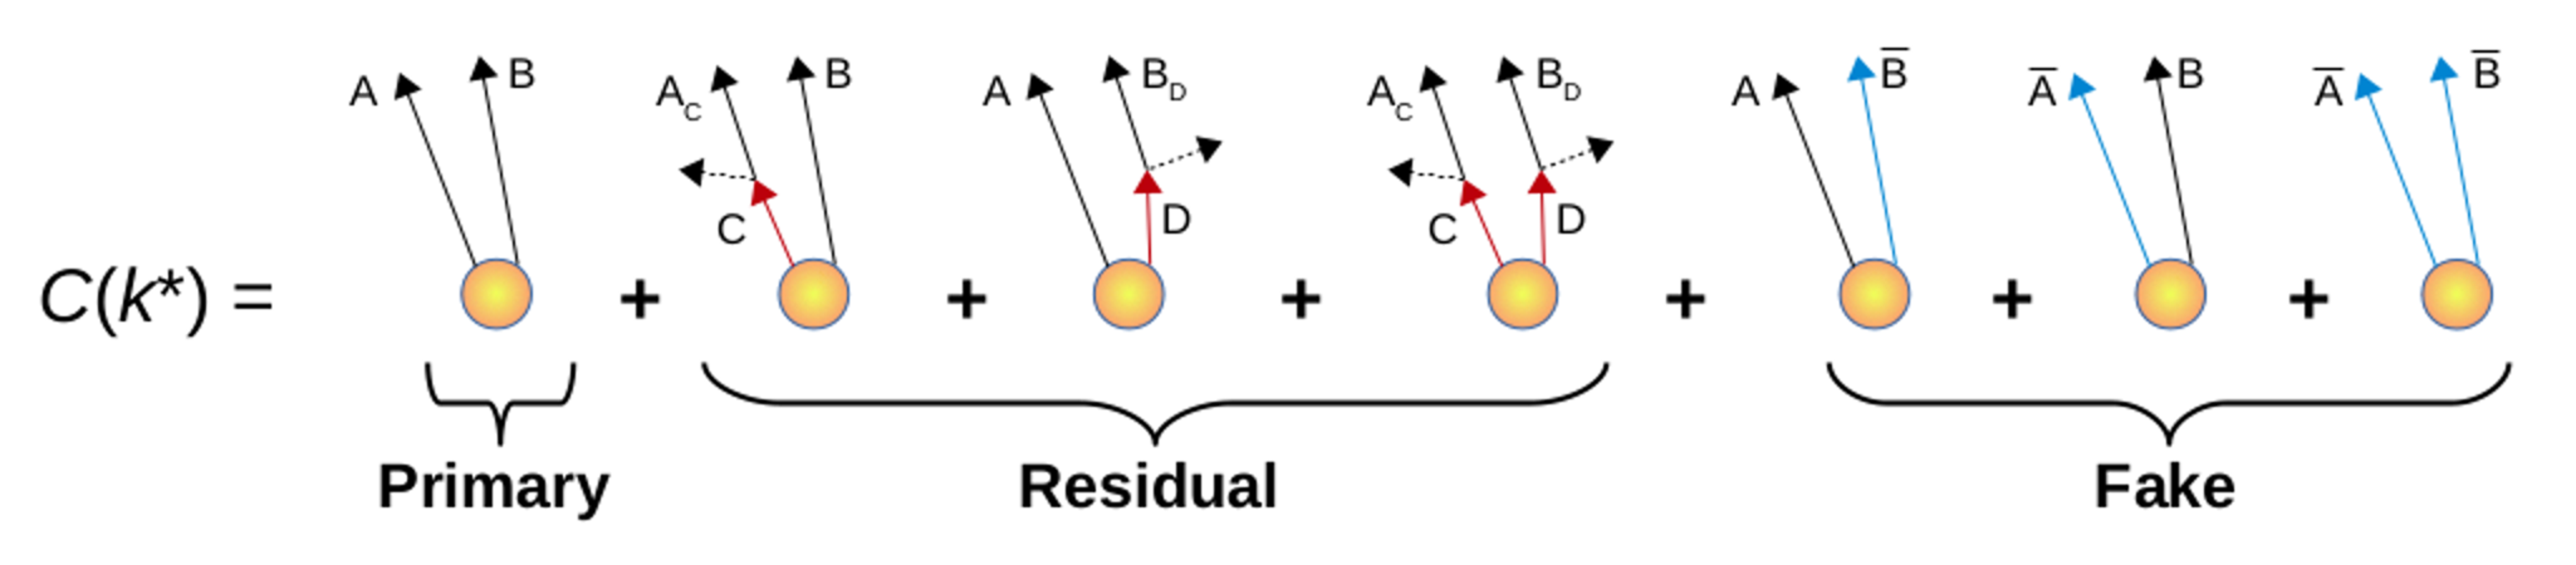
\includegraphics[width=\textwidth]{/home/jesse/Analysis/FemtoAnalysis/AnalysisNotes/5_Fitting/Figures/ResidualCartoons_p3.pdf}
  \caption[Residual Contributions Cartoon]{A schematic representation of the contributions to the finally measured data from the primary correlation, residual correlations, and fake pairs.}
  \label{fig:ResidualsCartoon}
\end{figure}


As it is difficult for us to eliminate these residual correlations in our analyses, we must attempt to account for them in our fit.
The genuine \LamK correlation function may be combined with the contributions from residual feed-down and misidentified particles to obtain the final, measured correlation function:


\begin{eqnarray}
\label{eqn:Residuals} 
 C_{\mathrm{measured}}(k^{*}_{\Lambda\mathrm{K}}) &=& 1 + \lambda'_{\Lambda\mathrm{K}}[C_{\Lambda\mathrm{K}}(k^{*}_{\Lambda\mathrm{K}}) - 1] + \sum\limits_{i,j}  \lambda'_{ij}[C_{ij}(k^{*}_{\Lambda\mathrm{K}})-1] \\
 \lambda_{ij}' &=& \lambda_{\mathrm{Fit}}\lambda_{ij} \notag \\
 \sum\limits_{i,j}\lambda_{ij}' &=&  \lambda_{\mathrm{Fit}}\sum\limits_{i,j}\lambda_{ij} = \lambda_{\mathrm{Fit}} \notag
\label{eqn:CfwRes} 
\end{eqnarray}

where the \LamK term represents the genuine \LamK correlation, and the $i$, $j$ terms denote the contributions from residual feed-down and possible impurities.
More specifically, $C_{ij}(k^{*}_{\Lambda\mathrm{K}})$ is the correlation function between parents of particle species $i$ and $j$, expressed in the basis of the relative momentum of the observed daughter \LamK pairs.  
The $\lambda$ parameters serve as weight dictating the strength of the parent contribution to the daughter pair, and are normalized to unity.
The individual $\lambda_{ij}$ are fixed (and whose values can be found in Table \ref{tab:LambdaValues_All}), but the parameter $\lambda_{\mathrm{Fit}}$ is left free.
The $\lambda_{\mathrm{Fit}}$ parameter serves as an overall normalization shared by all contributors.

In order to obtain the parent correlation function expressed in the relative momentum of the daughter pair, one must use a transform matrix.
The transform matrix describes the decay kinematics of the parent system into the daughter, and maps the \kstar of the parent pair onto that of the daughter.
Using this matrix, the transformed residual correlation function can be obtained:


\begin{equation}
  C_{ij}(k^{*}_{\Lambda\mathrm{K}}) \equiv \frac{\sum\limits_{k^{*}_{ij}} C_{ij}\left(k^{*}_{ij}\right) T\left(k^{*}_{ij},k^{*}_{\Lambda\mathrm{K}}\right)}{\sum\limits_{k^{*}_{ij}} T\left(k^{*}_{ij},k^{*}_{\Lambda\mathrm{K}}\right)}
\label{eqn:ResidualsTransform}
\end{equation}


The transform matrix is generated with the THERMINATOR 2 \cite{Chojnacki:2011hb} simulation. 
It is formed for a given parent pair, $ij$, by taking all \LamK pairs originating from $ij$, calculating the relative momentum of the parents ($k^{*}_{ij}$) and daughters ($k^{*}_{\Lambda\mathrm{K}}$), and filling a two-dimensional histogram with the values. 
The transform matrix is essentially an unnormalized probability distribution mapping the \kstar of the parent pair to that of the daughter pair when one or both parents decay.
An example of such transform matrices can be found in Figures \ref{fig:TransformMatricesLamKchP} and \ref{fig:TransformMatricesALamKchP}.

\begin{figure}[h!]
  \centering
  %%----start of first subfigure---  
  \subfloat[Transform matrix for $\Sigma$K$^{+}$ pairs into $\Lambda$K$^{+}$]{
    \label{fig:TransformMatricesLamKchP:a}
    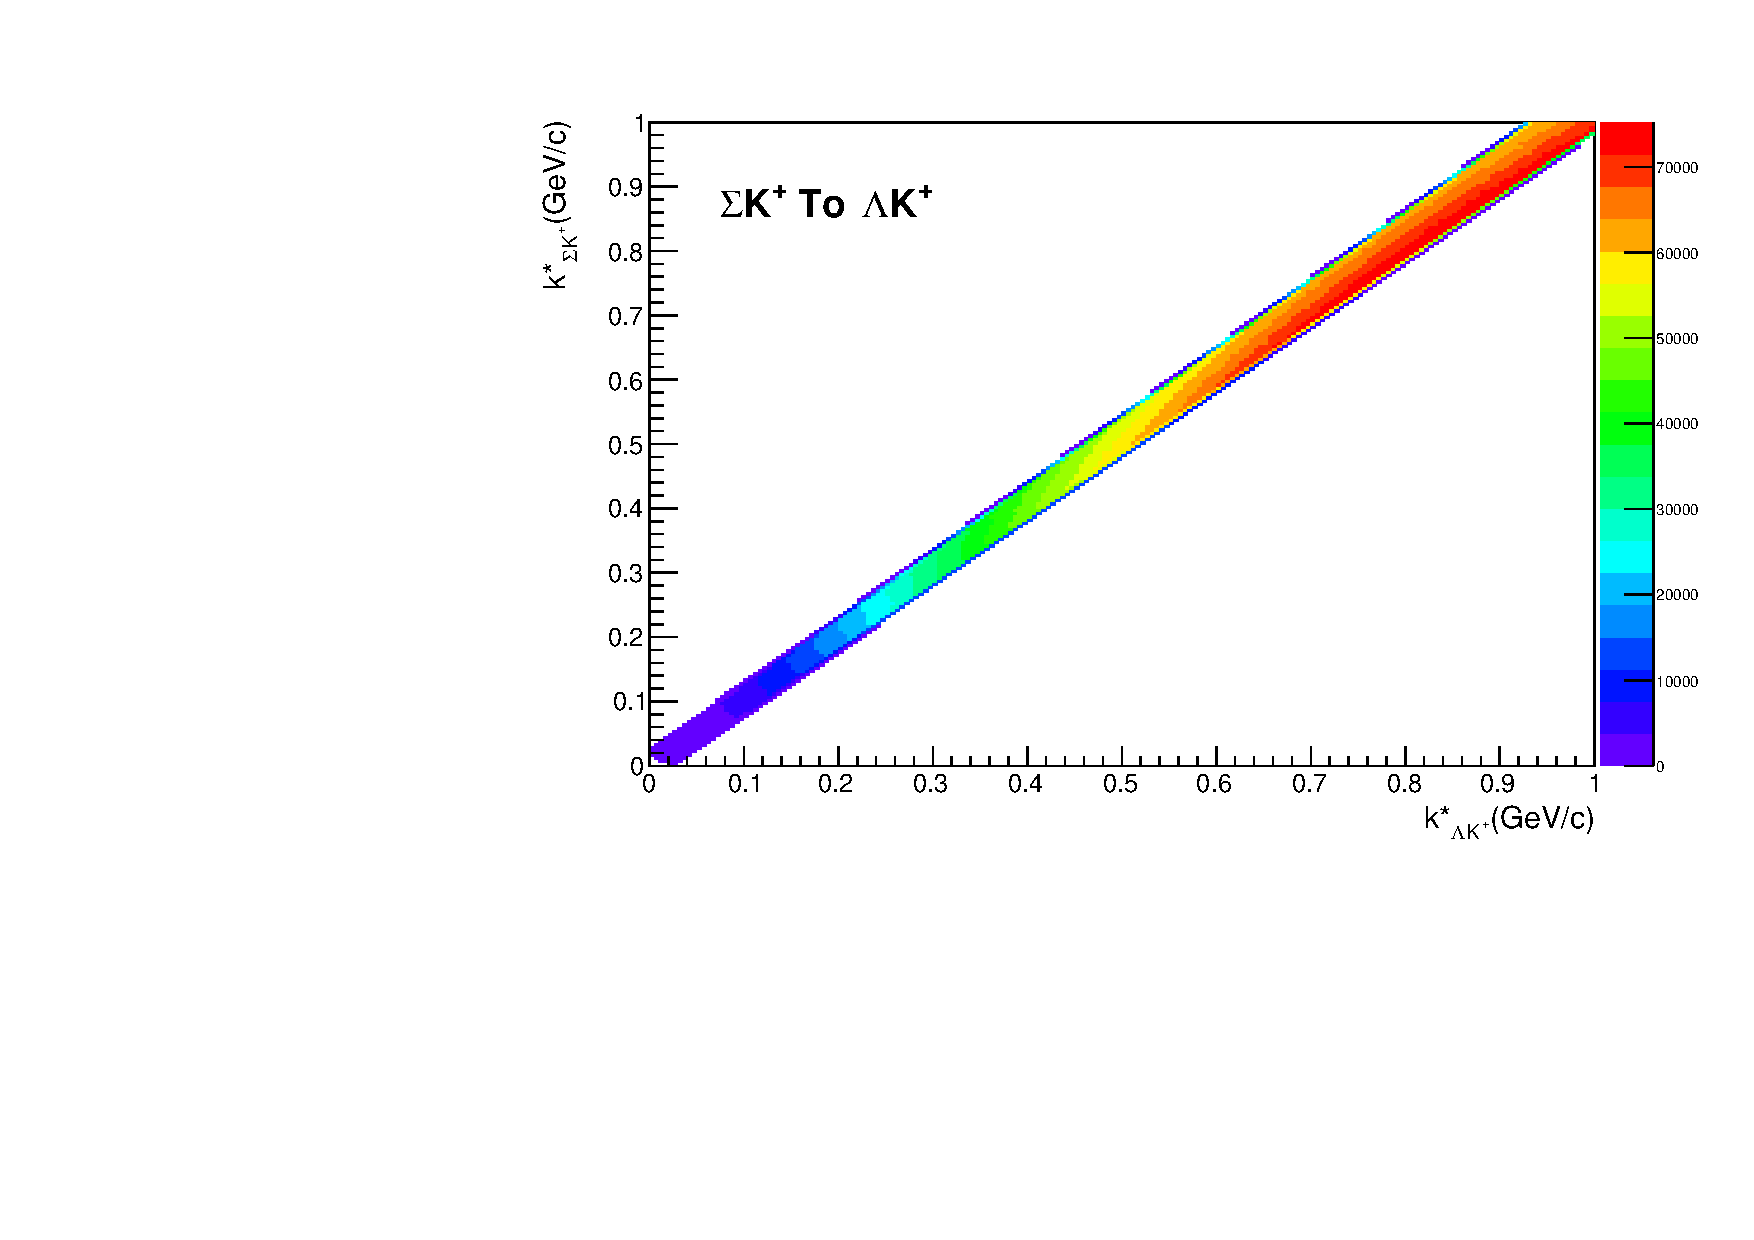
\includegraphics[width=0.49\textwidth]{/home/jesse/Analysis/FemtoAnalysis/AnalysisNotes/5_Fitting/Figures/fSigToLamKchPTransform.pdf}}%\\
  %%----start of second subfigure---
  \subfloat[Transform matrix for $\Xi^{-}$K$^{+}$ pairs into $\Lambda$K$^{+}$]{
    \label{fig:TransformMatricesLamKchP:b}
    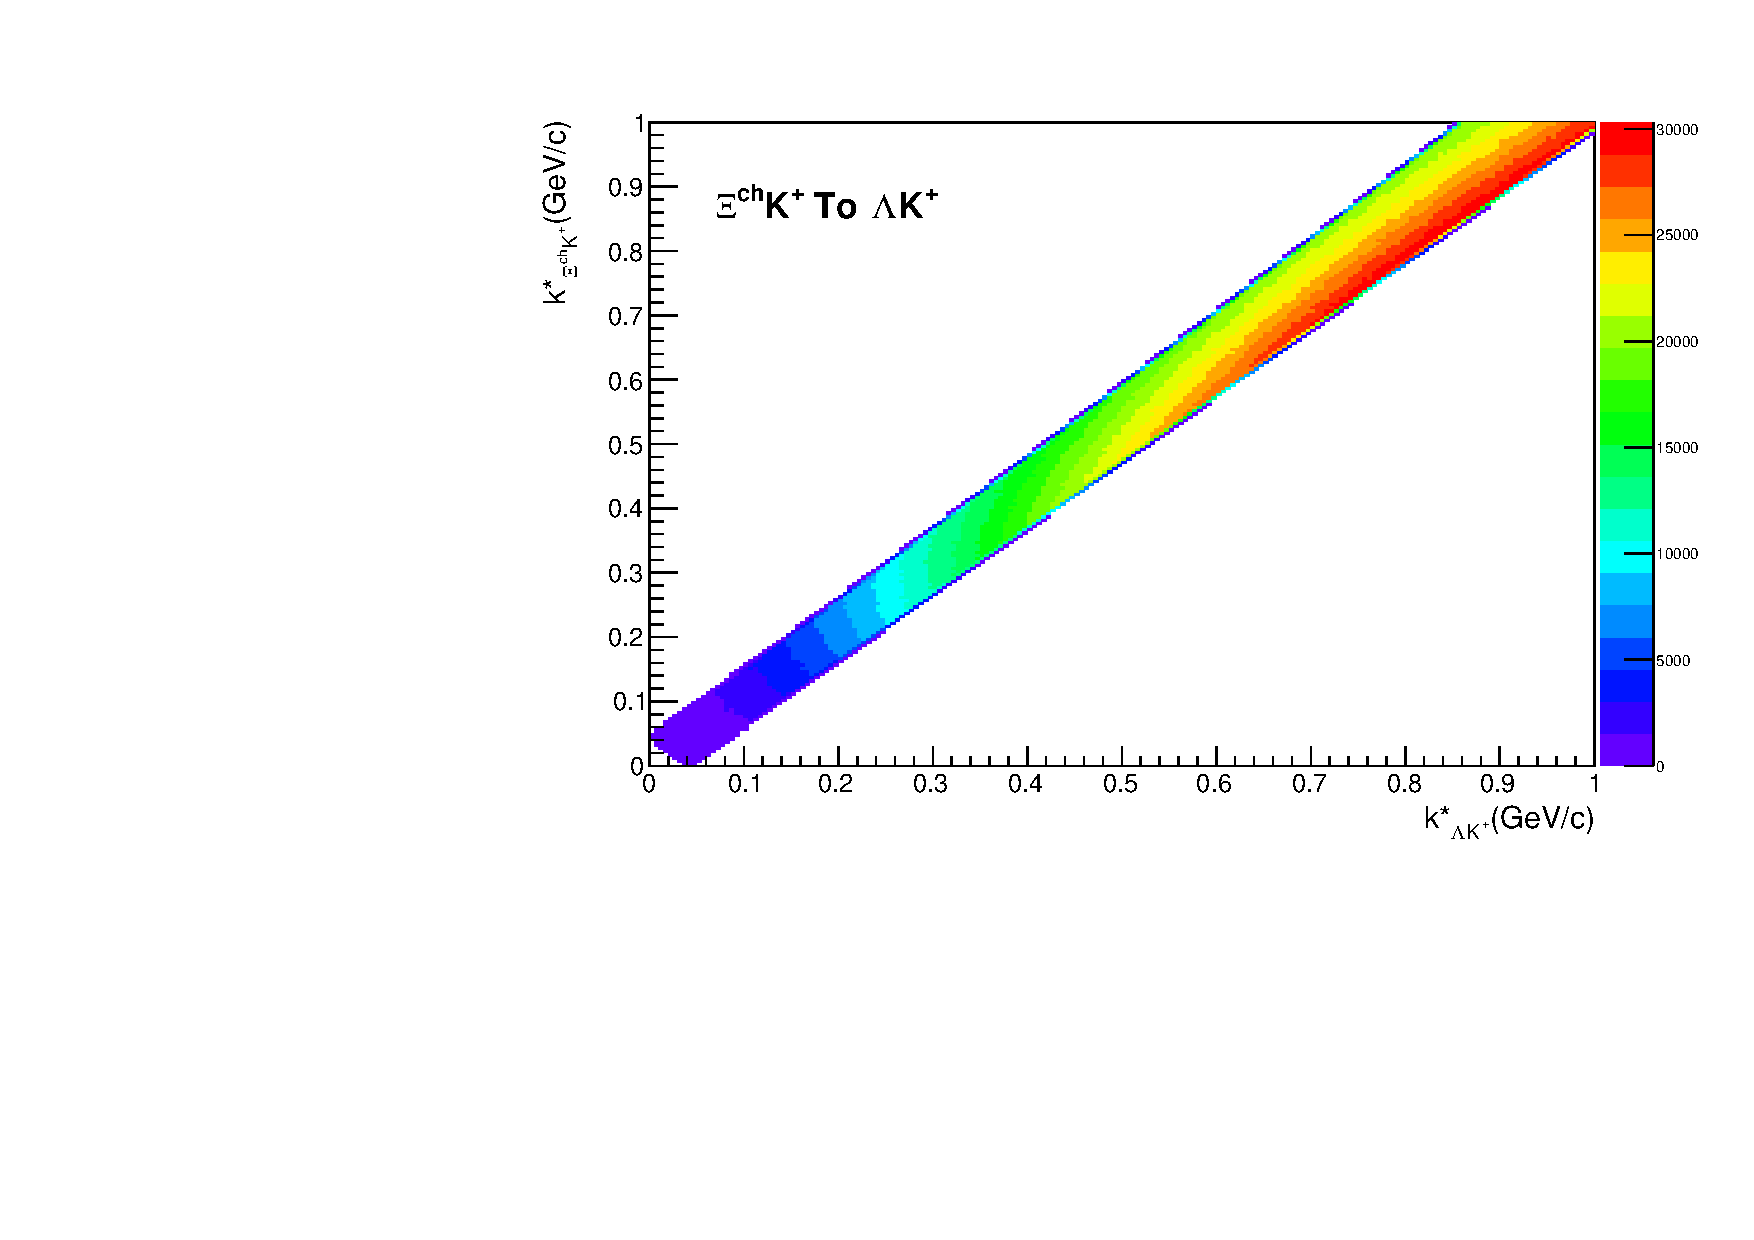
\includegraphics[width=0.49\textwidth]{/home/jesse/Analysis/FemtoAnalysis/AnalysisNotes/5_Fitting/Figures/fXiCToLamKchPTransform.pdf}} \\
  %%----start of third subfigure---
  \subfloat[Transform matrix for $\Xi^{0}$K$^{+}$ pairs into $\Lambda$K$^{+}$]{
    \label{fig:TransformMatricesLamKchP:c}
    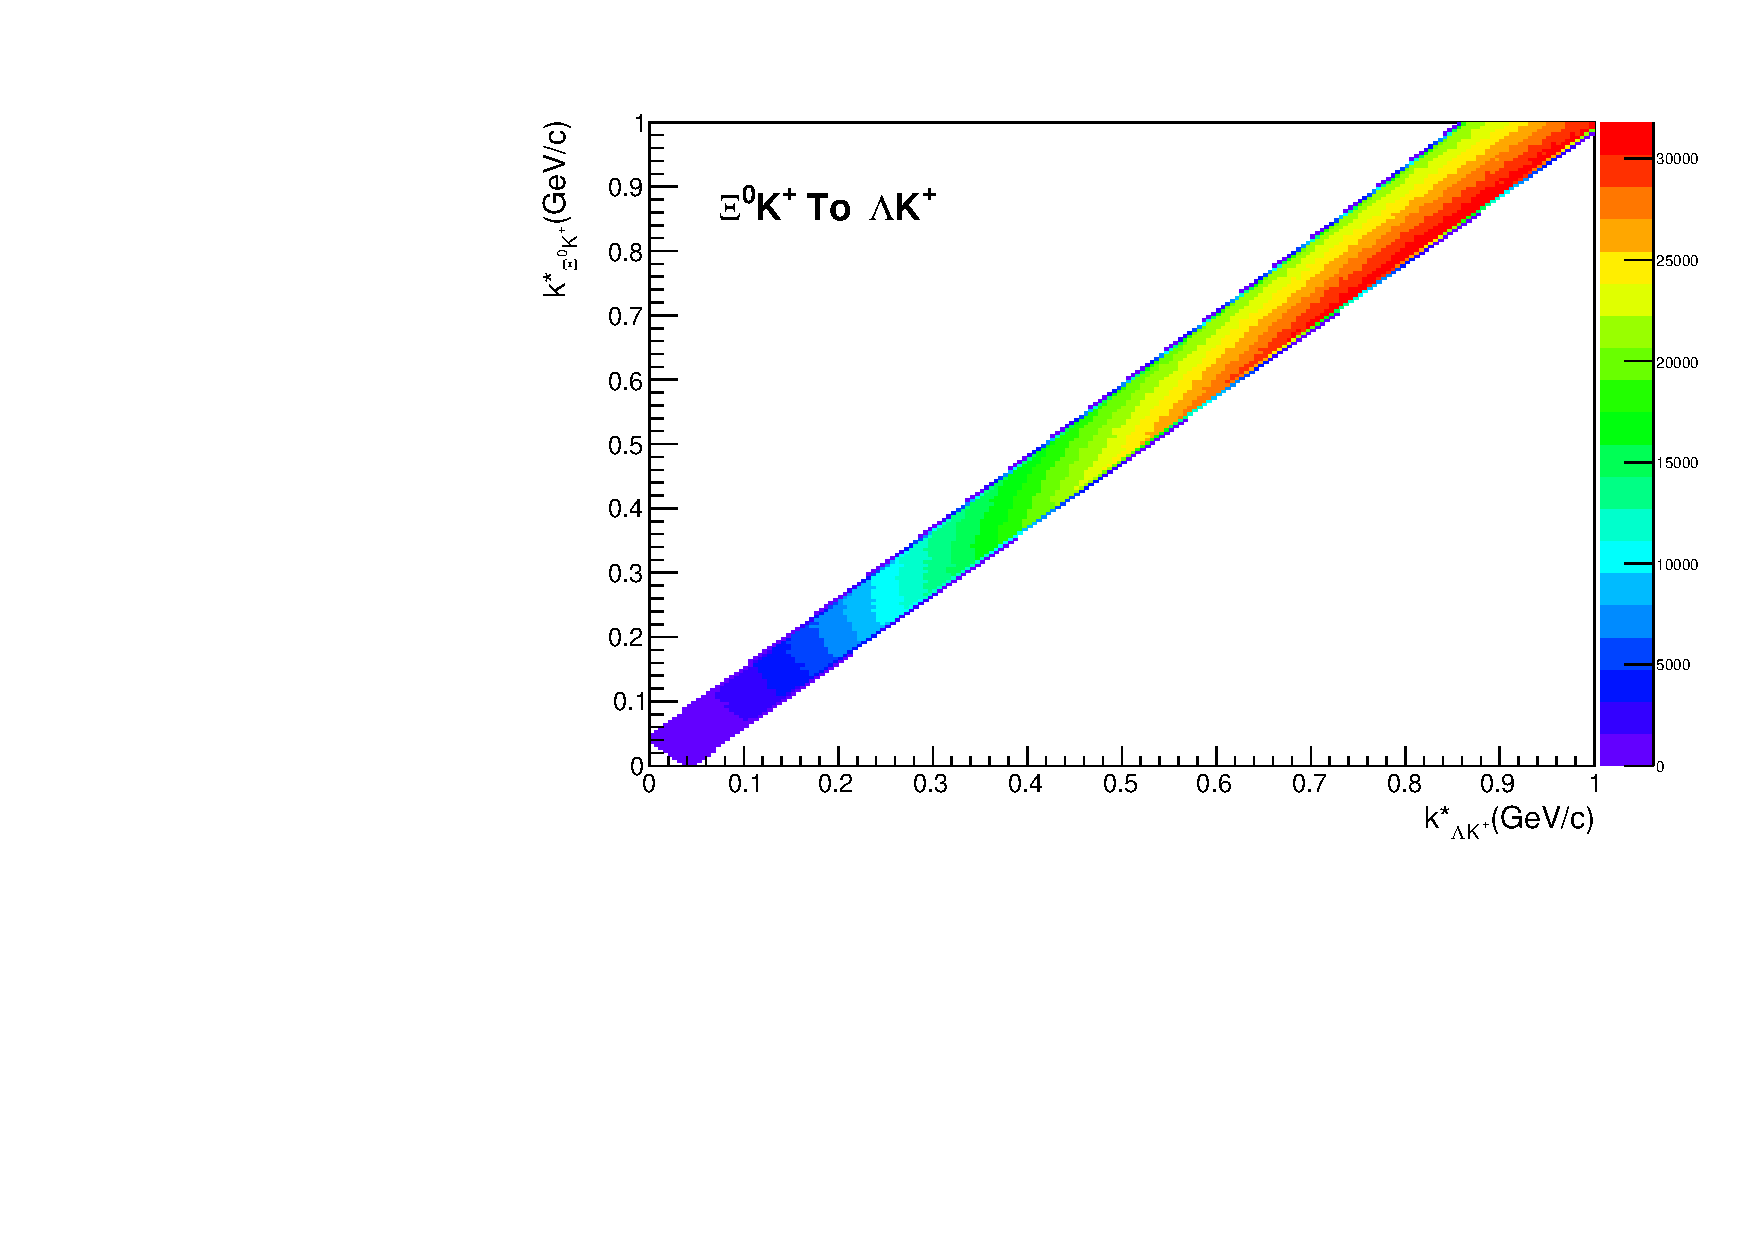
\includegraphics[width=0.49\textwidth]{/home/jesse/Analysis/FemtoAnalysis/AnalysisNotes/5_Fitting/Figures/fXi0ToLamKchPTransform.pdf}}
  %%----start of fourth subfigure---
  \subfloat[Transform matrix for $\Omega^{-}$K$^{+}$ pairs into $\Lambda$K$^{+}$]{
    \label{fig:TransformMatricesLamKchP:d}
    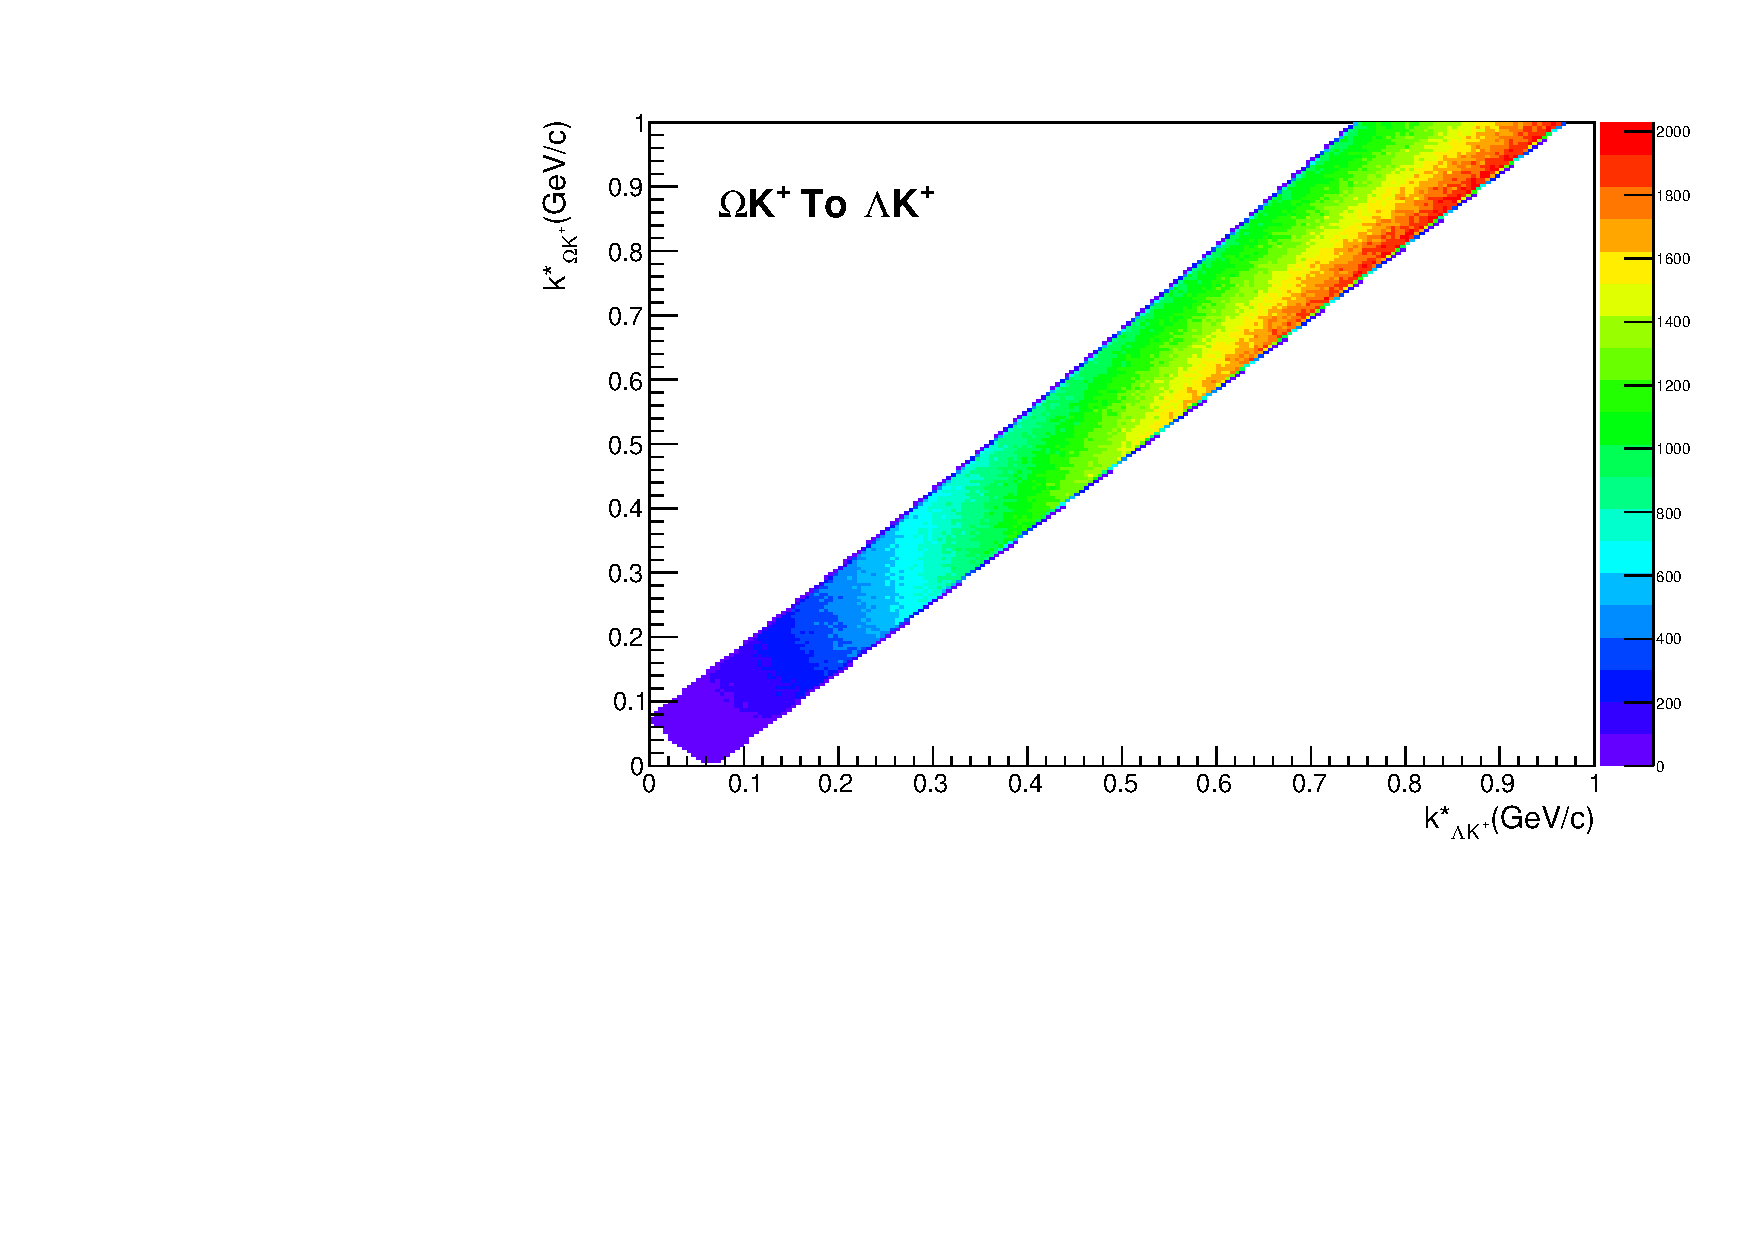
\includegraphics[width=0.49\textwidth]{/home/jesse/Analysis/FemtoAnalysis/AnalysisNotes/5_Fitting/Figures/fOmegaToLamKchPTransform.pdf}} \\                   
  %%----overall caption----
  \caption[Sample Transform Matrices for \LamKchP Analysis]{Sample Transform Matrices generated with THERMINATOR for \LamKchP Analysis}
  \label{fig:TransformMatricesLamKchP}
\end{figure}


\begin{figure}[h!]
  \centering
  %%----start of first subfigure---
  \subfloat[Transform matrix for $\bar{\Sigma}$K$^{+}$ pairs into $\bar{\Lambda}$K$^{+}$]{
    \label{fig:TransformMatricesALamKchP:a}
    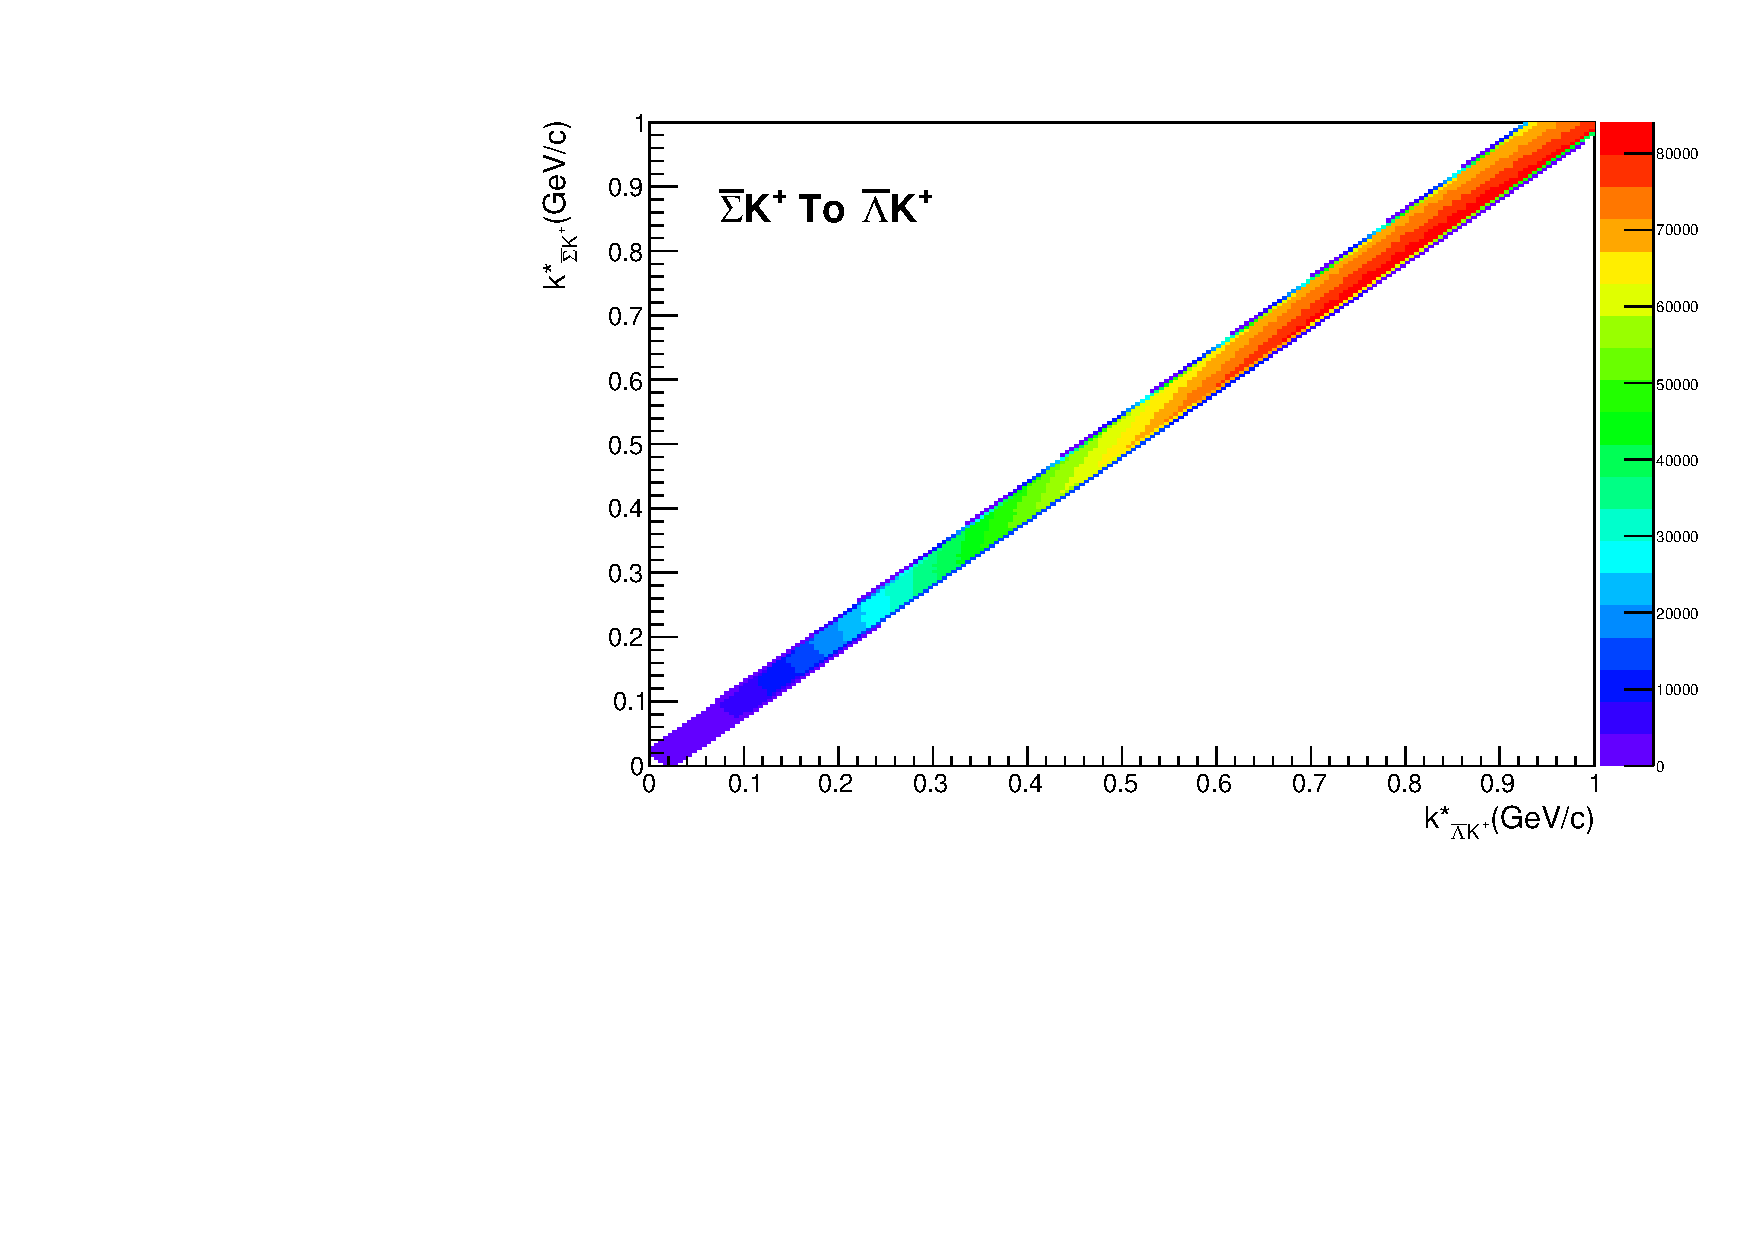
\includegraphics[width=0.49\textwidth]{/home/jesse/Analysis/FemtoAnalysis/AnalysisNotes/5_Fitting/Figures/fASigToALamKchPTransform.pdf}}
  %%----start of second subfigure---
  \subfloat[Transform matrix for $\bar{\Xi}^{+}$K$^{+}$ pairs into $\bar{\Lambda}$K$^{+}$]{
    \label{fig:TransformMatricesALamKchP:b}
    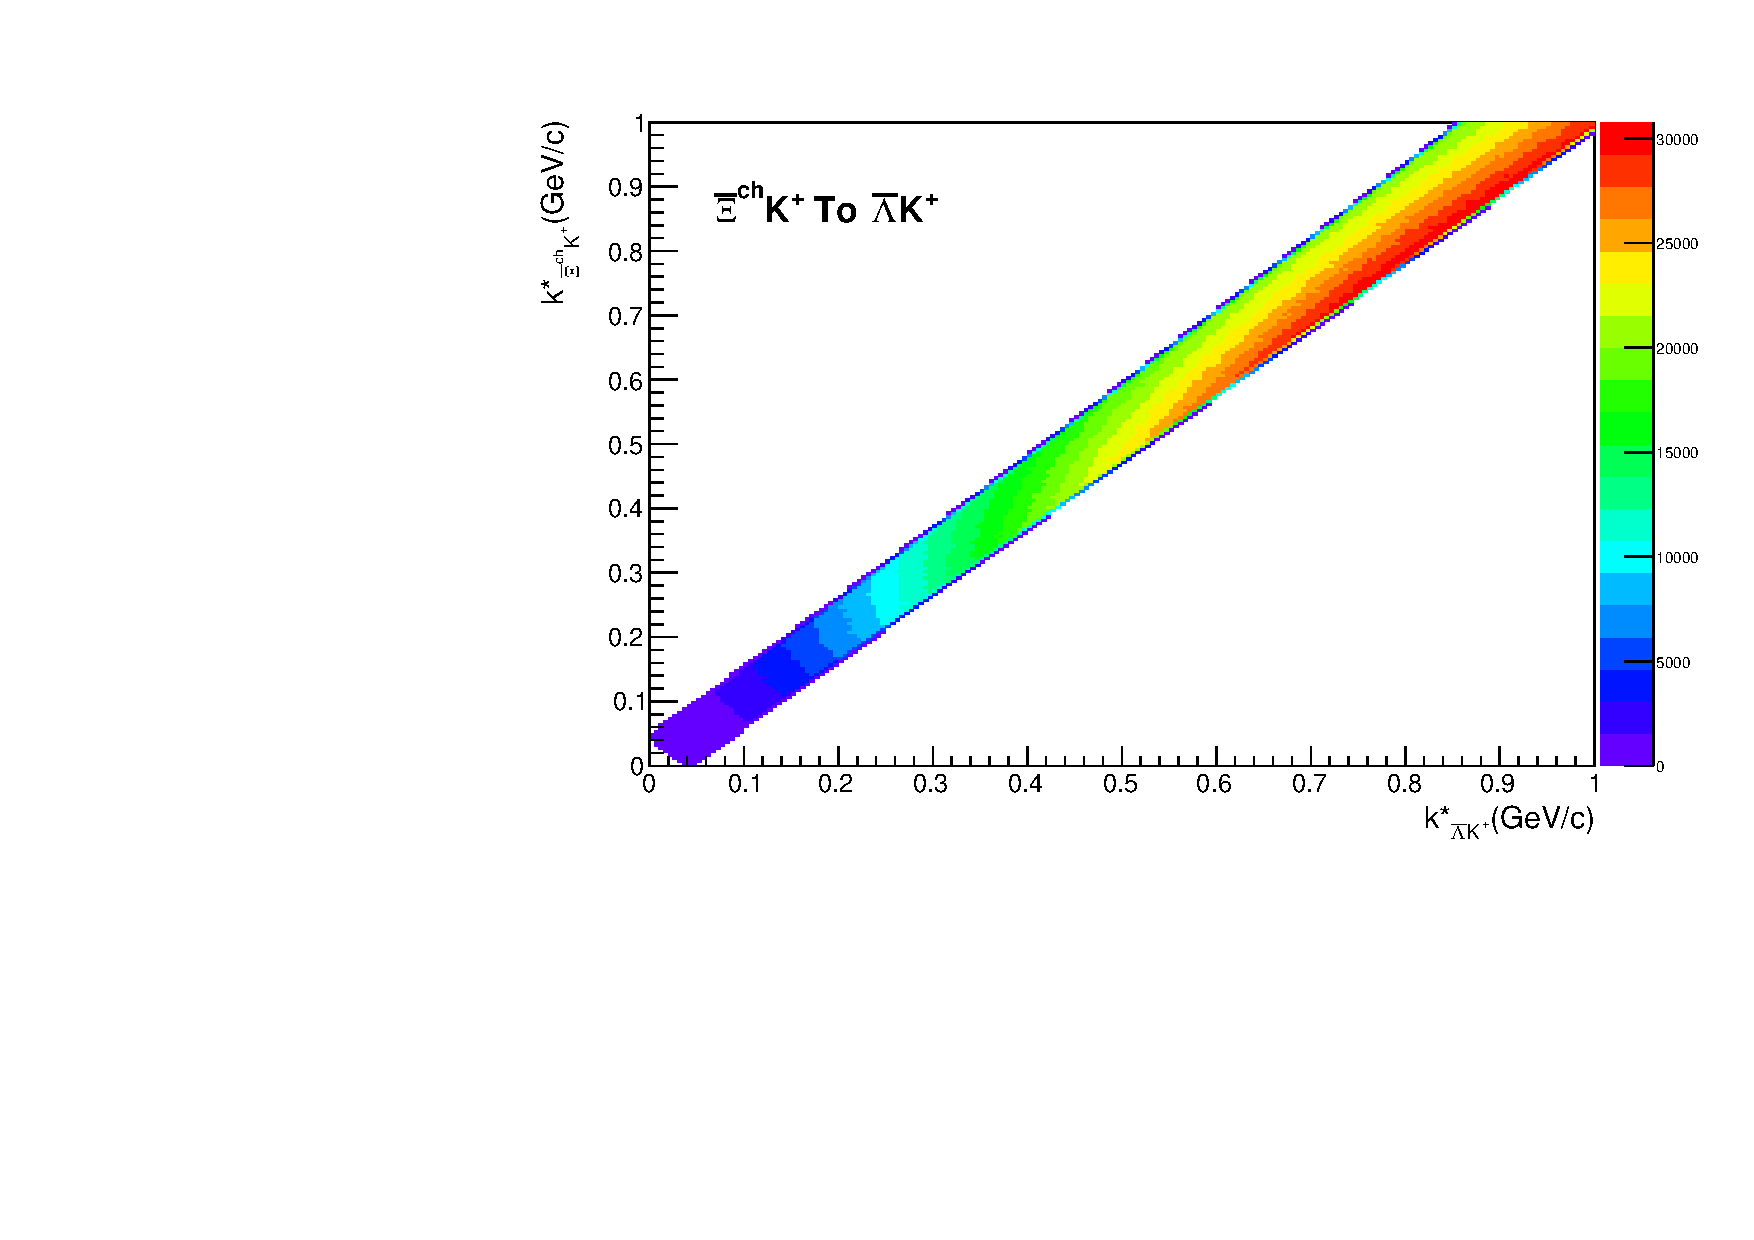
\includegraphics[width=0.49\textwidth]{/home/jesse/Analysis/FemtoAnalysis/AnalysisNotes/5_Fitting/Figures/fAXiCToALamKchPTransform.pdf}} \\
  %%----start of third subfigure---
  \subfloat[Transform matrix for $\bar{\Xi}^{0}$K$^{+}$ pairs into $\bar{\Lambda}$K$^{+}$]{
    \label{fig:TransformMatricesALamKchP:c}
    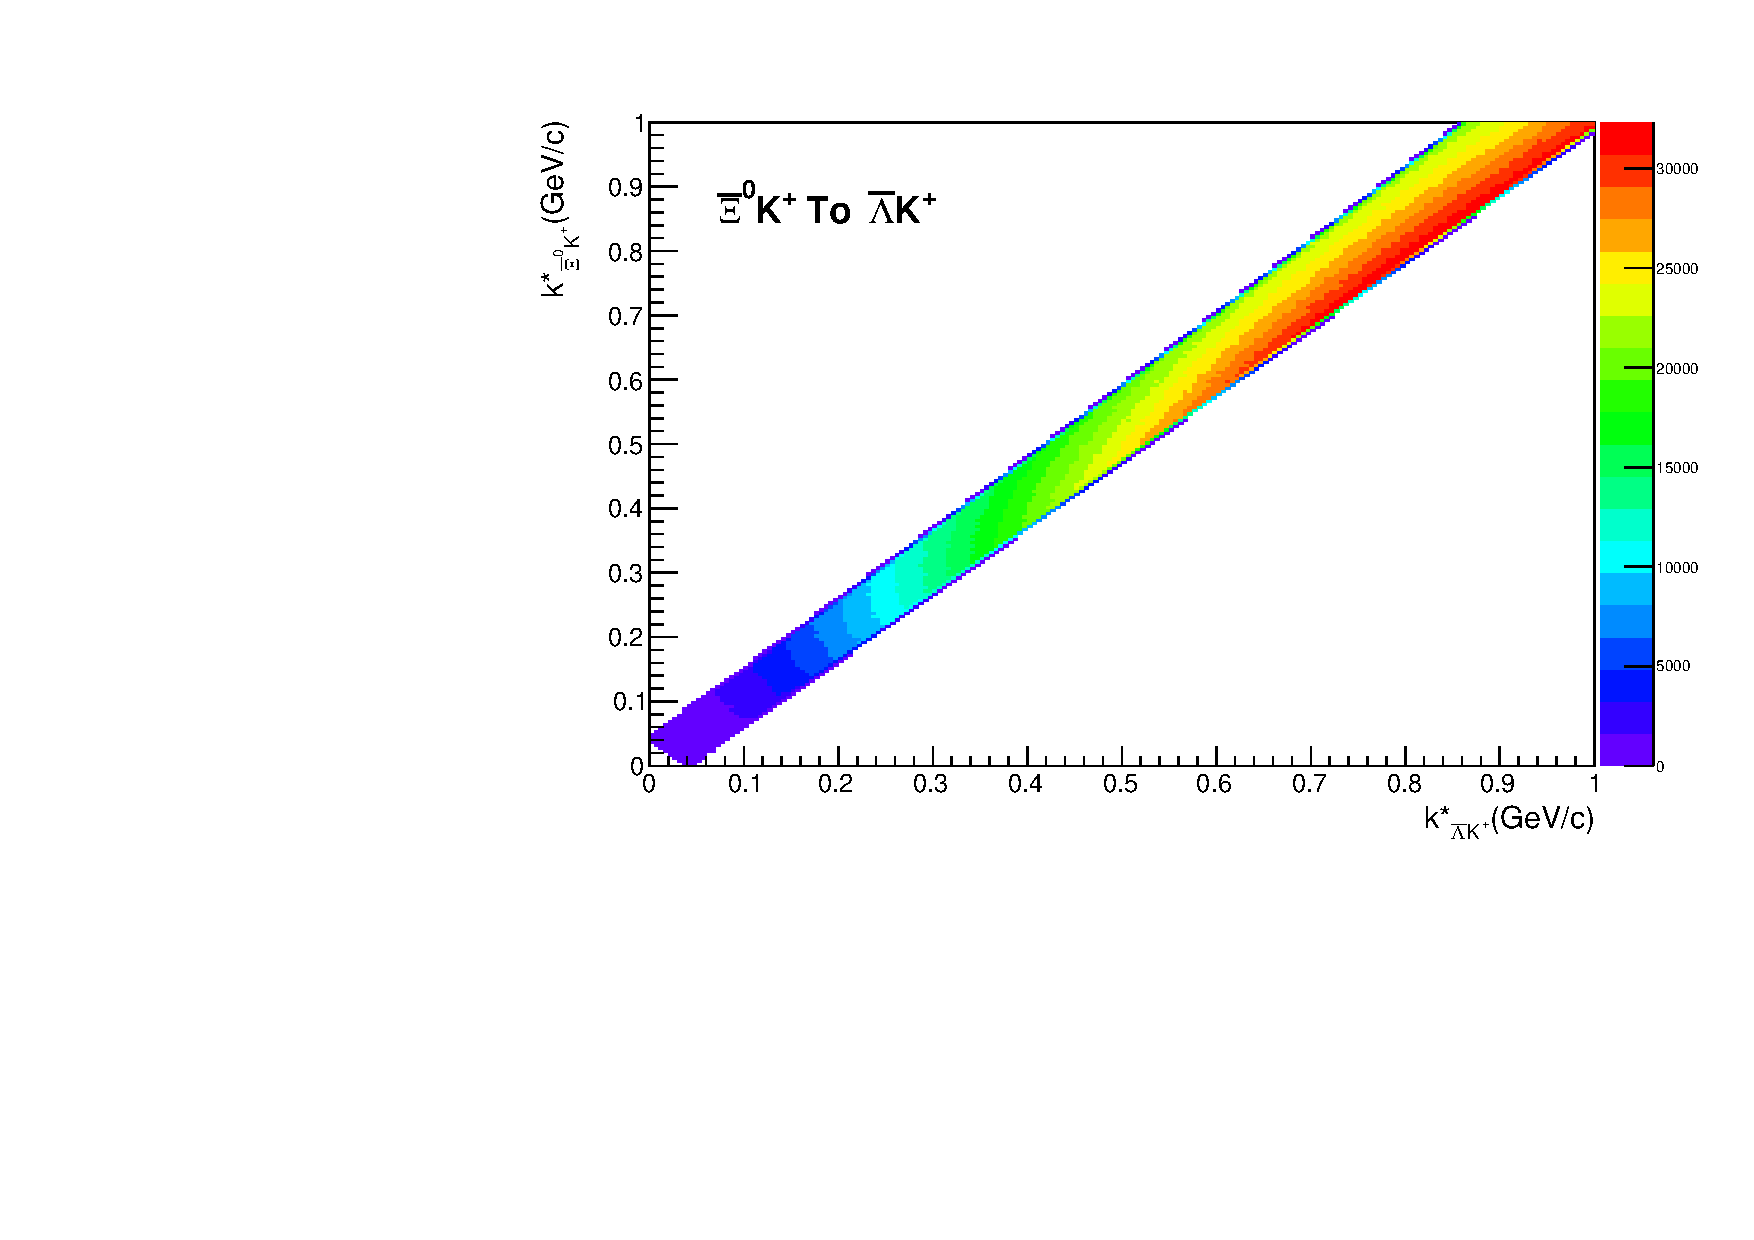
\includegraphics[width=0.49\textwidth]{/home/jesse/Analysis/FemtoAnalysis/AnalysisNotes/5_Fitting/Figures/fAXi0ToALamKchPTransform.pdf}}
  %%----start of fourth subfigure---
  \subfloat[Transform matrix for $\bar{\Omega}^{+}$K$^{+}$ pairs into $\bar{\Lambda}$K$^{+}$]{
    \label{fig:TransformMatricesALamKchP:d}
    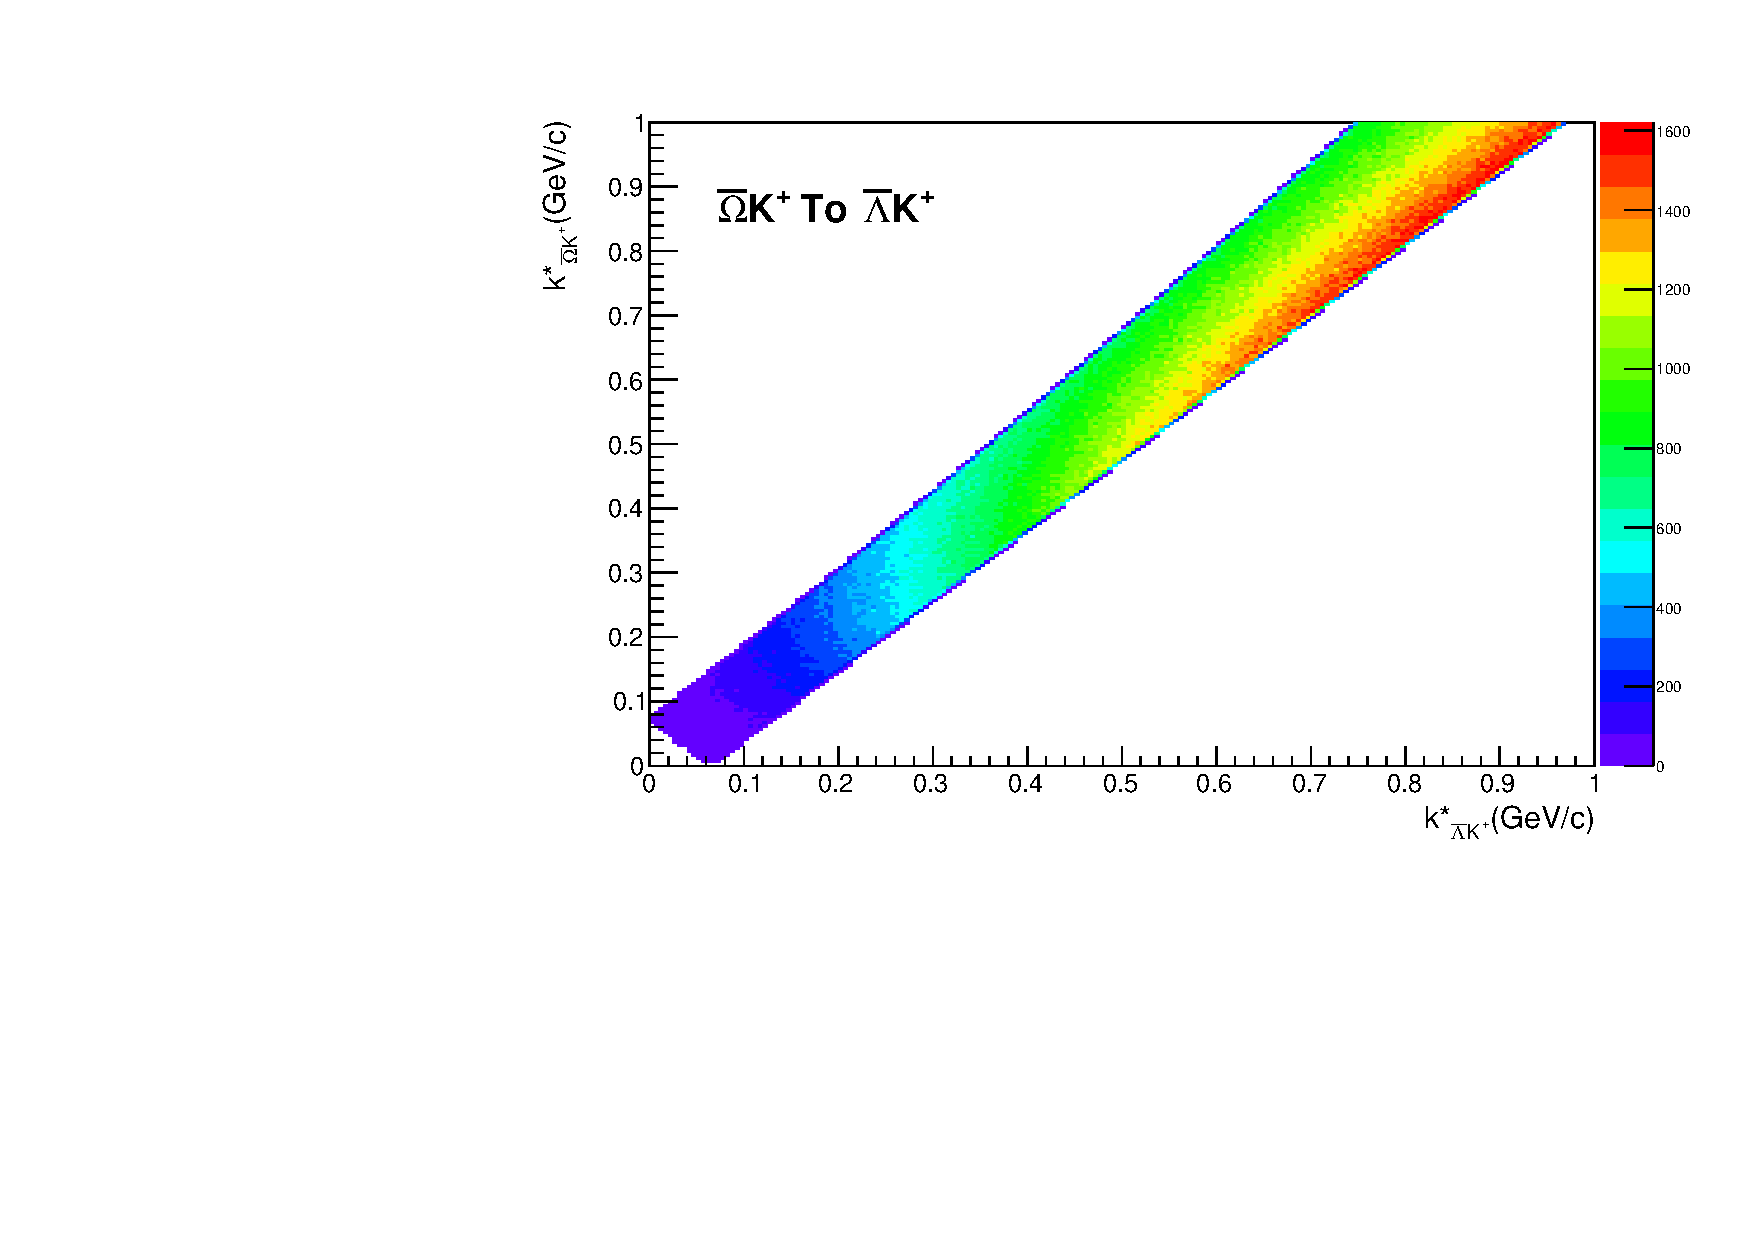
\includegraphics[width=0.49\textwidth]{/home/jesse/Analysis/FemtoAnalysis/AnalysisNotes/5_Fitting/Figures/fAOmegaToALamKchPTransform.pdf}}                    
  %%----overall caption----
  \caption[Sample Transform Matrices for \ALamKchP Analysis]{Sample Transform Matrices generated with THERMINATOR for \ALamKchP Analysis}
  \label{fig:TransformMatricesALamKchP}
\end{figure}


Femtoscopic analyses are sensitive to the pair emission structure at kinetic freeze-out.
Therefore, in the eyes of femtoscopy, any particle born from a resonance decay before last rescattering is seen as primary.
For our study, when including three residual contributors, we consider a particle to be primary if its parent has a proper decay length of $c\tau <$ 10 fm.
When including ten residual contributors, we must reduce this number to $c\tau <$ 4 fm for consistency.
Moving to ten contributors, we introduce feed-down from $\Sigma^{*}$ and K$^{*}$ resonances, with proper decay lengths of $c\tau \approx$ 5 fm and $c\tau \approx$ 4 fm, respectively.
As these are considered non-primary for the case of ten contributors, so must any resonance with $c\tau >$ 4 fm.

 
As previously stated, the $\lambda$ parameters dictate the strength of the parent contribution to the daughter pair.  
Therefore, the $\lambda$ parameter for parent system AB can be estimated as the total number of $\Lambda$K pairs in our experimental sample originating from AB (N$_{AB}$) divided by the total number of $\Lambda$K pairs (N$_{Total}$):

\begin{equation}
\lambda_{AB} = \frac{N_{AB}}{N_{Total}}
\end{equation}

The particle yields can be estimated using THERMINATOR 2 simulation ($N_{ij}^{\scaleto{THERM}{3pt}}$), while the reconstruction efficiencies ($RE_{ij}$) are estimated with MC HIJING data, which has been run through GEANT to simulate the detector response (Fig. \ref{fig:RecoEffs}).  Thus, the $\lambda$ parameters are estimated as:

\begin{equation}
\lambda_{AB} = \frac{N_{AB}}{N_{Total}} = \frac{N_{AB}^{\scaleto{THERM}{3pt}}RE_{AB}^{\scaleto{HIJING}{3pt}}}{\sum\limits_{ij} N_{ij}^{\scaleto{THERM}{3pt}}RE_{ij}^{\scaleto{HIJING}{3pt}}}
\end{equation}

\begin{figure}[h!]
  \centering
  %%----start of first subfigure---
  \subfloat[Reconstruction Efficiencies (3 Residuals)]{
    \label{fig:RecoEffs_3Res}
    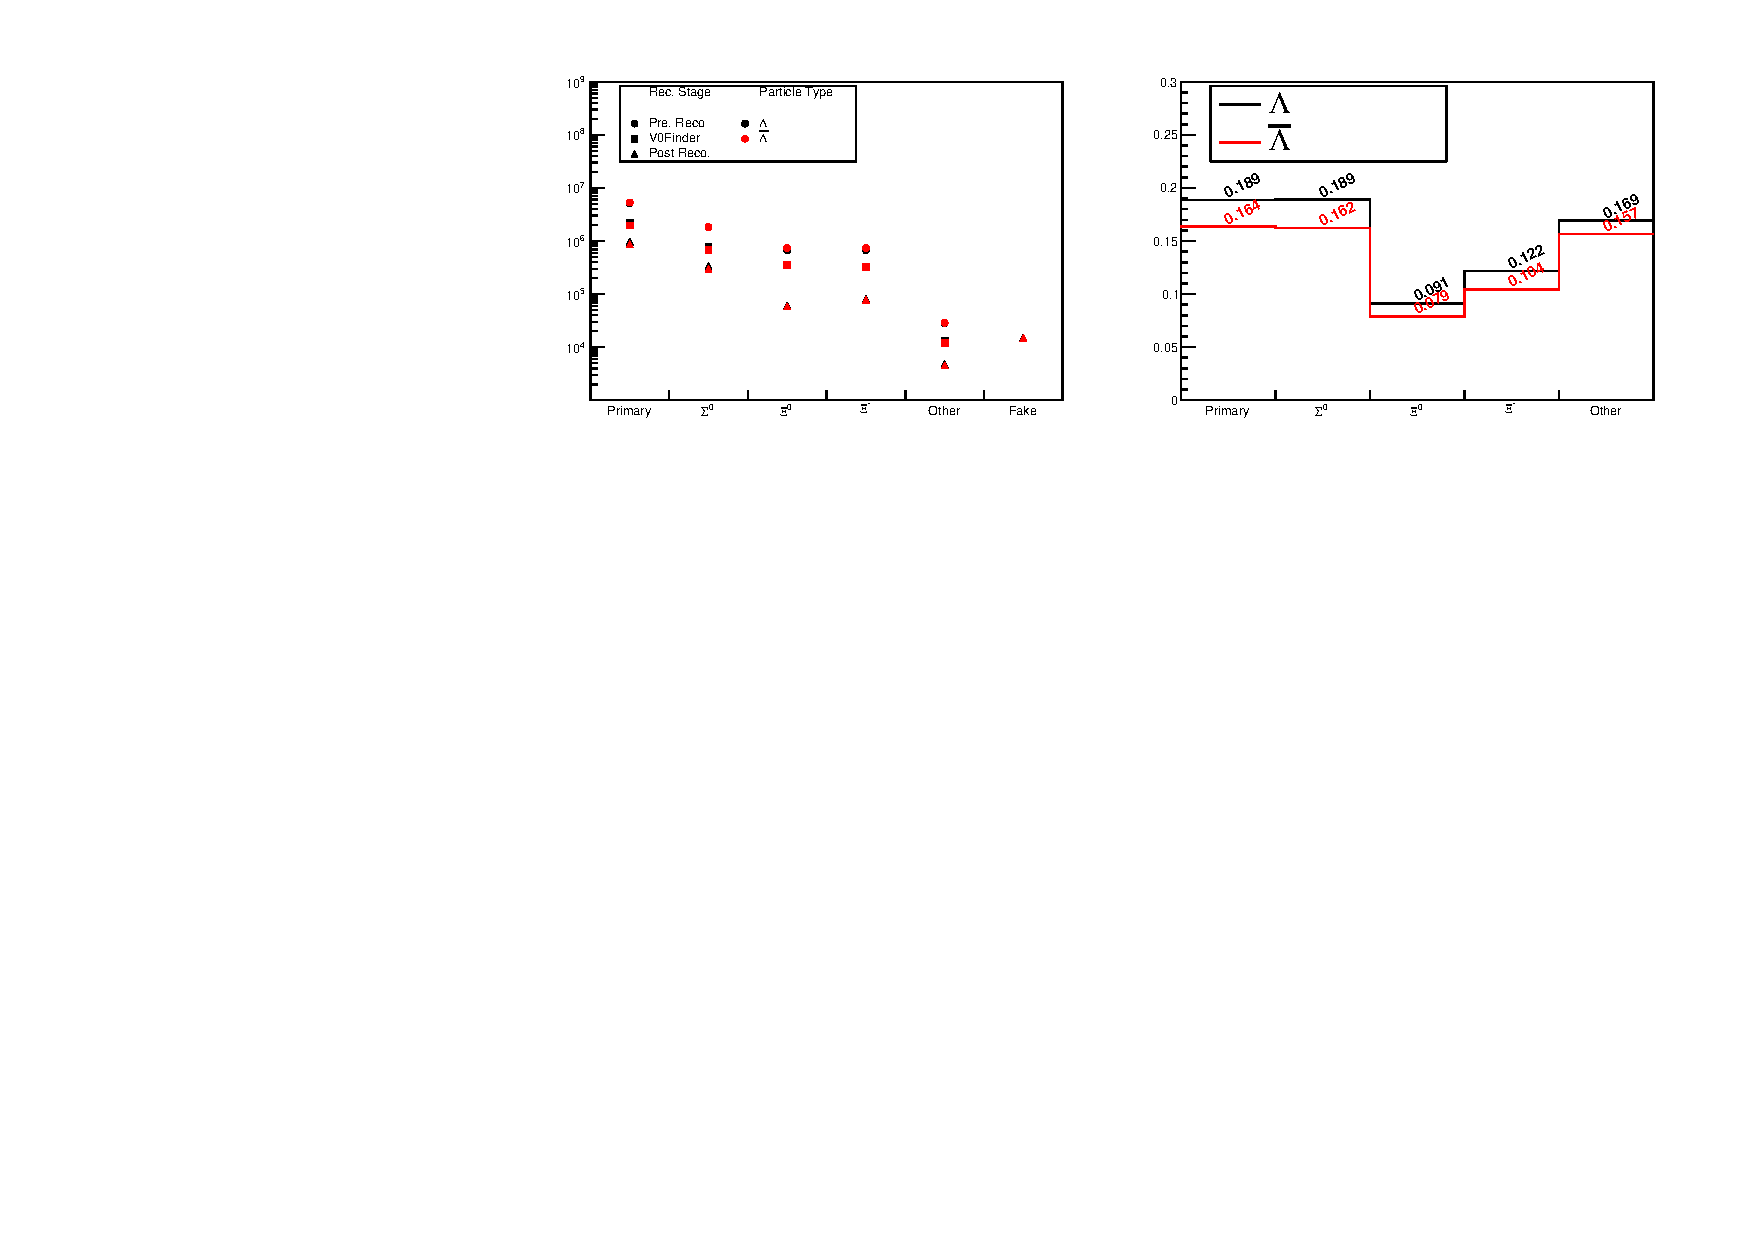
\includegraphics[width=\textwidth]{\VZeroEffDirBase 20181024/tCanTruthsAndEffs_woInjected_Built_3Res_MaxDecay10_wV0Finder_Pretty.pdf}} \\
  %%----start of second subfigure---
  \subfloat[Reconstruction Efficiencies (10 Residuals)]{
    \label{fig:RecoEffs_10Res}
    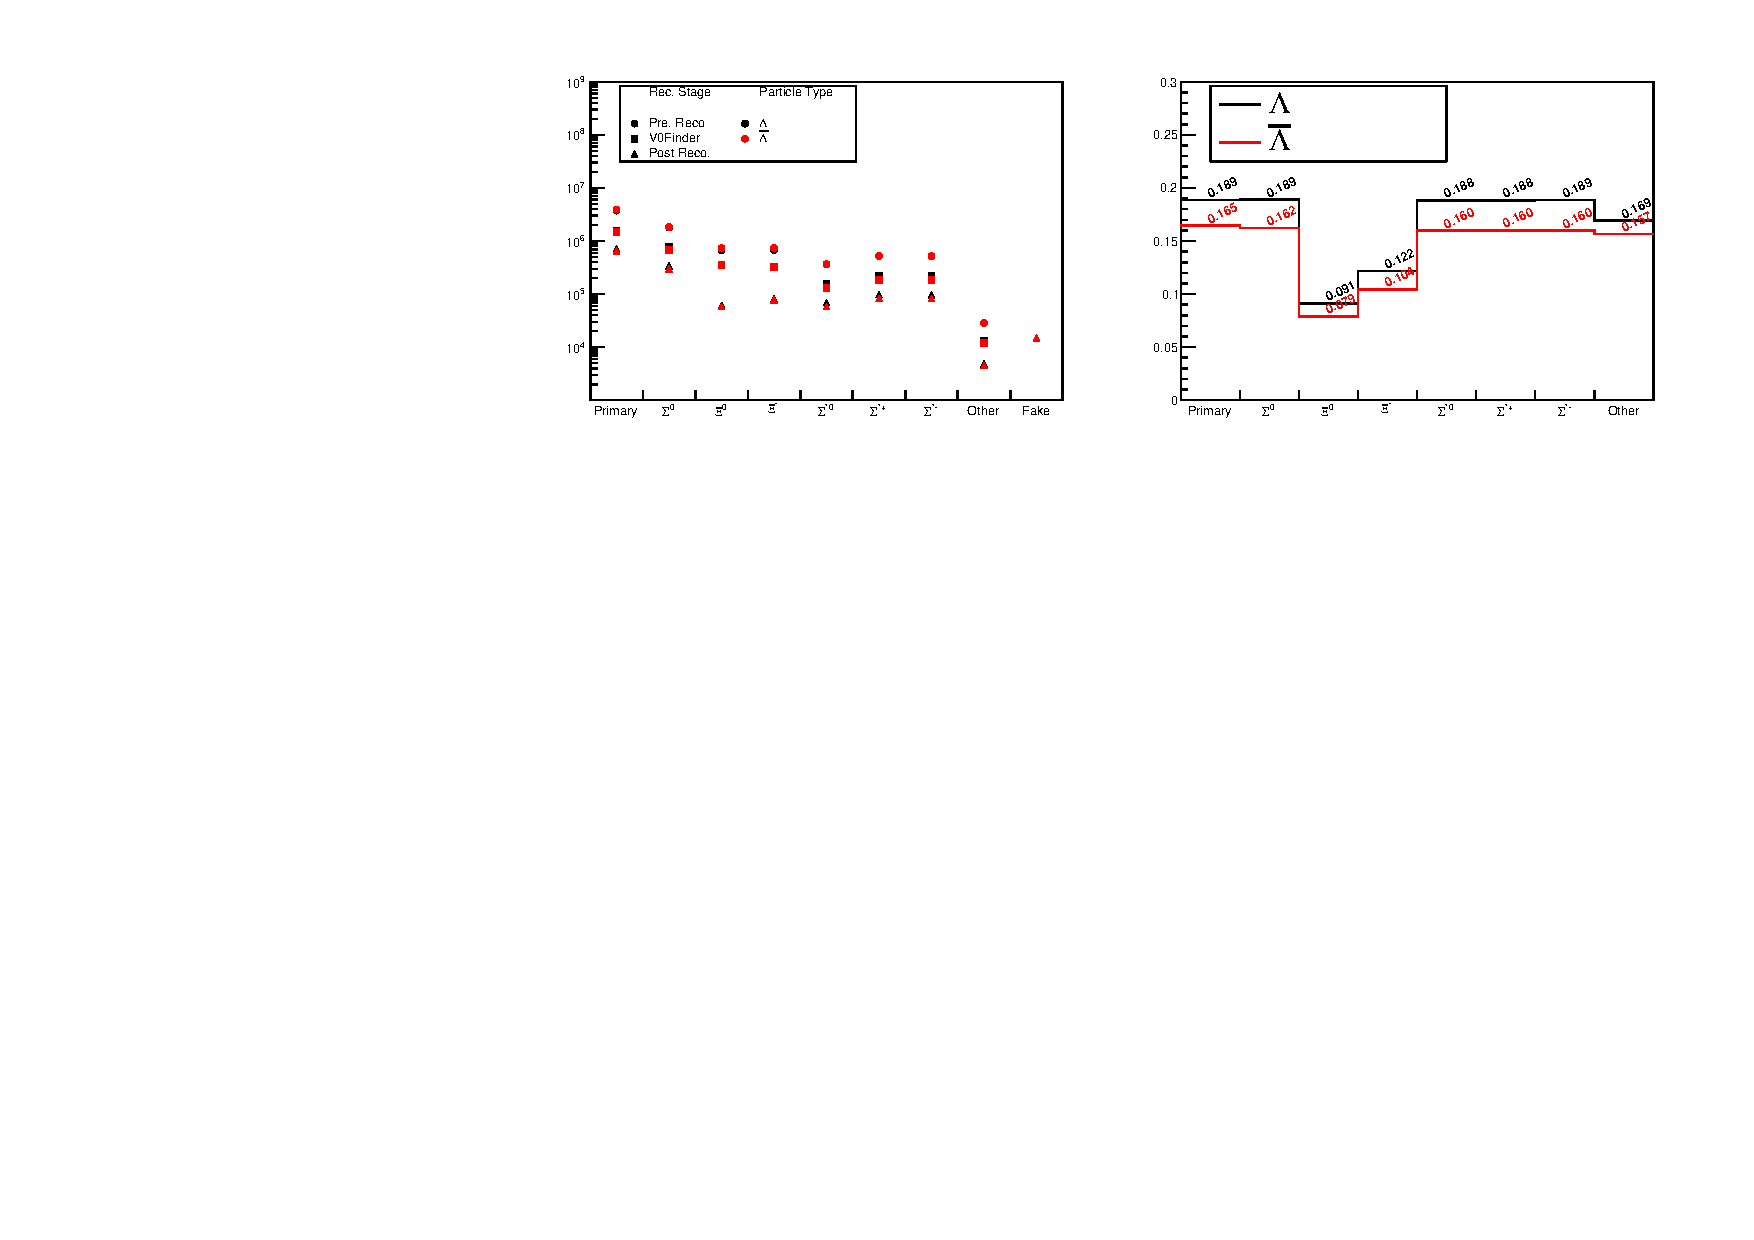
\includegraphics[width=\textwidth]{\VZeroEffDirBase 20181024/tCanTruthsAndEffs_woInjected_Built_10Res_MaxDecay4_wV0Finder_Pretty.pdf}}                 
  %%----overall caption----
  \caption[Reconstruction Efficiencies]{Reconstruction Efficiencies}
  \label{fig:RecoEffs}
\end{figure}

The $\lambda$ values used can be found in Table \ref{tab:LambdaValues_All}, for the case of both three and ten residual contributors.  In the table, we also list the $\lambda$ values used for ``Other'' and ``Fakes''.  The ``Other'' category contains pairs which are not primary, and which do not originate from the (3 or 10) residual pairs included in the fit.  The ``Fakes'' category represents pairs that are mistakenly identified as \LamK.  To estimate this $\lambda_{\mathrm{Fakes}}$ value, we assumed that the number of fake pairs was equal to the total number of pairs multiplied by the \Lam purity (i.e. assuming perfect purity for the kaons); or, more simply, $\lambda_{\mathrm{Fakes}}$ = 1.0 - Purity(\Lam).  For both of these contributors (``Other'' and ``Fakes''), we assume that these correlations average to unity, and therefore do not contribute to the final correlation function.

%%%%%%%%%%%%%%%%%%%%%%%%%%%%%%%%%%%%%%%%%%%%%%%%%%%%%%%%%%%%%%%%%%%%%%%%%%%%%%%%%%%%%%%%%%%%%
\pagestyle{empty}
\begin{landscape}

\begin{table}[htbp]
 \centering
 \renewcommand{\arraystretch}{1.2}
 \resizebox{\paperwidth}{!}{
 \begin{tabular}{|c|cV{5.0}c|cV{5.0}c|cV{5.0}c|cV{5.0}c|cV{5.0}c|c|}
  \multicolumn{2}{c}{\LamKchP residuals} & \multicolumn{2}{c}{\ALamKchM residuals} & \multicolumn{2}{c}{\LamKchM residuals} & \multicolumn{2}{c}{\ALamKchP residuals} & \multicolumn{2}{c}{\LamKs residuals} & \multicolumn{2}{c}{\ALamKs residuals} \\
  \hline
  \textbf{Pair System} & \textbf{$\lambda$ value} & \textbf{Pair System} & \textbf{$\lambda$ value} & \textbf{Pair System} & \textbf{$\lambda$ value} & \textbf{Pair System} & \textbf{$\lambda$ value} & \textbf{Pair System} & \textbf{$\lambda$ value} & \textbf{Pair System} & \textbf{$\lambda$ value} \\
  \hlineB{3.0}
  \multicolumn{12}{|c|}{3 Residuals (Max Parent $c\tau_{\mathrm{decay}}$ = 10 fm)} \\
  \hlineB{3.0}
  $\Lambda$K$^{+}$ & 0.527 & $\bar{\Lambda}$K$^{-}$ & 0.526 & $\Lambda$K$^{-}$ & 0.526 & $\bar{\Lambda}$K$^{+}$ & 0.527 & $\Lambda$K$^{0}_{\mathrm{S}}$ & 0.543 & $\bar{\Lambda}$K$^{0}_{\mathrm{S}}$ & 0.544 \\
  
  $\Sigma^{0}$K$^{+}$ & 0.111 & $\bar{\Sigma}^{0}$K$^{-}$ & 0.110 & $\Sigma^{0}$K$^{-}$ & 0.110 & $\bar{\Sigma}^{0}$K$^{+}$ & 0.111 & $\Sigma^{0}$K$^{0}_{\mathrm{S}}$ & 0.120 & $\bar{\Sigma}^{0}$K$^{0}_{\mathrm{S}}$ & 0.120 \\
  
  $\Xi^{0}$K$^{+}$ & 0.039 & $\bar{\Xi}^{0}$K$^{-}$ & 0.035 & $\Xi^{0}$K$^{-}$ & 0.038 & $\bar{\Xi}^{0}$K$^{+}$ & 0.036 & $\Xi^{0}$K$^{0}_{\mathrm{S}}$ & 0.042 & $\bar{\Xi}^{0}$K$^{0}_{\mathrm{S}}$ & 0.039 \\
  
  $\Xi^{-}$K$^{+}$ & 0.050 & $\bar{\Xi}^{+}$K$^{-}$ & 0.046 & $\Xi^{-}$K$^{-}$ & 0.050 & $\bar{\Xi}^{+}$K$^{+}$ & 0.046 & $\Xi^{-}$K$^{0}_{\mathrm{S}}$ & 0.054 & $\bar{\Xi}^{+}$K$^{0}_{\mathrm{S}}$ & 0.050 \\
  
  Other & 0.226 & Other & 0.235 & Other & 0.228 & Other & 0.233 & Other & 0.194 & Other & 0.199 \\
  
  Fakes & 0.048 & Fakes & 0.048 & Fakes & 0.048 & Fakes & 0.048 & Fakes & 0.048 & Fakes & 0.048 \\
  
  \hlineB{3.0}  
  \multicolumn{12}{|c|}{10 Residuals (Max Parent $c\tau_{\mathrm{decay}}$ = 4 fm)} \\
  \hlineB{3.0}
  $\Lambda$K$^{+}$ & 0.180 & $\bar{\Lambda}$K$^{-}$ & 0.180 & $\Lambda$K$^{-}$ & 0.179 & $\bar{\Lambda}$K$^{+}$ & 0.181 & $\Lambda$K$^{0}_{\mathrm{S}}$ & 0.192 & $\bar{\Lambda}$K$^{0}_{\mathrm{S}}$ & 0.193 \\
  
  $\Sigma^{0}$K$^{+}$ & 0.116 & $\bar{\Sigma}^{0}$K$^{-}$ & 0.114 & $\Sigma^{0}$K$^{-}$ & 0.115 & $\bar{\Sigma}^{0}$K$^{+}$ & 0.116 & $\Sigma^{0}$K$^{0}_{\mathrm{S}}$ & 0.125 & $\bar{\Sigma}^{0}$K$^{0}_{\mathrm{S}}$ & 0.124 \\
  
  $\Xi^{0}$K$^{+}$ & 0.040 & $\bar{\Xi}^{0}$K$^{-}$ & 0.037 & $\Xi^{0}$K$^{-}$ & 0.040 & $\bar{\Xi}^{0}$K$^{+}$ & 0.037 & $\Xi^{0}$K$^{0}_{\mathrm{S}}$ & 0.043 & $\bar{\Xi}^{0}$K$^{0}_{\mathrm{S}}$ & 0.040 \\
  
  $\Xi^{-}$K$^{+}$ & 0.052 & $\bar{\Xi}^{+}$K$^{-}$ & 0.047 & $\Xi^{-}$K$^{-}$ & 0.052 & $\bar{\Xi}^{+}$K$^{+}$ & 0.048 & $\Xi^{-}$K$^{0}_{\mathrm{S}}$ & 0.056 & $\bar{\Xi}^{+}$K$^{0}_{\mathrm{S}}$ & 0.052 \\
  
  $\Sigma^{*+}$K$^{+}$ & 0.054 & $\bar{\Sigma}^{*-}$K$^{-}$ & 0.051 & $\Sigma^{*+}$K$^{-}$ & 0.053 & $\bar{\Sigma}^{*-}$K$^{+}$ & 0.051 & $\Sigma^{*+}$K$^{0}_{\mathrm{S}}$ & 0.058 & $\bar{\Sigma}^{*-}$K$^{0}_{\mathrm{S}}$ & 0.055 \\
  
  $\Sigma^{*-}$K$^{+}$ & 0.048 & $\bar{\Sigma}^{*+}$K$^{-}$ & 0.050 & $\Sigma^{*-}$K$^{-}$ & 0.048 & $\bar{\Sigma}^{*+}$K$^{+}$ & 0.050 & $\Sigma^{*-}$K$^{0}_{\mathrm{S}}$ & 0.052 & $\bar{\Sigma}^{*+}$K$^{0}_{\mathrm{S}}$ & 0.054 \\
  
  $\Sigma^{*0}$K$^{+}$ & 0.048 & $\bar{\Sigma}^{*0}$K$^{-}$ & 0.045 & $\Sigma^{*0}$K$^{-}$ & 0.048 & $\bar{\Sigma}^{*0}$K$^{+}$ & 0.045 & $\Sigma^{*0}$K$^{0}_{\mathrm{S}}$ & 0.052 & $\bar{\Sigma}^{*0}$K$^{0}_{\mathrm{S}}$ & 0.048 \\
  
  $\Lambda$K$^{*0}$ & 0.046 & $\bar{\Lambda}\bar{\mathrm{K}}^{*0}$ & 0.047 & $\Lambda\bar{\mathrm{K}}^{*0}$ & 0.046 & $\bar{\Lambda}$K$^{*0}$ & 0.047 & $\Lambda$K$^{*0}$ & 0.022 & $\bar{\Lambda}$K$^{*0}$ & 0.022 \\
  
  $\Sigma^{0}$K$^{*0}$ & 0.041 & $\bar{\Sigma}^{0}\bar{\mathrm{K}}^{*0}$ & 0.041 & $\Sigma^{0}\bar{\mathrm{K}}^{*0}$ & 0.041 & $\bar{\Sigma}^{0}$K$^{*0}$ & 0.041 & $\Sigma^{0}$K$^{*0}$ & 0.019 & $\bar{\Sigma}^{0}$K$^{*0}$ & 0.019 \\
  
  $\Xi^{0}$K$^{*0}$ & 0.014 & $\bar{\Xi}^{0}\bar{\mathrm{K}}^{*0}$ & 0.013 & $\Xi^{0}\bar{\mathrm{K}}^{*0}$ & 0.014 & $\bar{\Xi}^{0}$K$^{*0}$ & 0.013 & $\Xi^{0}$K$^{*0}$ & 0.007 & $\bar{\Xi}^{0}$K$^{*0}$ & 0.006 \\
  
  $\Xi^{-}$K$^{*0}$ & 0.018 & $\bar{\Xi}^{+}\bar{\mathrm{K}}^{*0}$ & 0.017 & $\Xi^{-}\bar{\mathrm{K}}^{*0}$ & 0.018 & $\bar{\Xi}^{+}$K$^{*0}$ & 0.017 & $\Xi^{-}$K$^{*0}$ & 0.009 & $\bar{\Xi}^{+}$K$^{*0}$ & 0.008 \\
  
  Other & 0.295 & Other & 0.310 & Other & 0.299 & Other & 0.307 & Other & 0.318 & Other & 0.330 \\
  
  Fakes & 0.048 & Fakes & 0.048 & Fakes & 0.048 & Fakes & 0.048 & Fakes & 0.048 & Fakes & 0.048 \\
  
  \hlineB{3.0}
 \end{tabular}}
 \caption{$\lambda$ values for the individual components of the \LamK correlation functions for the case of 3 and 10 residual contributions.}
 \label{tab:LambdaValues_All}
\end{table}

\end{landscape}
\pagestyle{plain}
%%%%%%%%%%%%%%%%%%%%%%%%%%%%%%%%%%%%%%%%%%%%%%%%%%%%%%%%%%%%%%%%%%%%%%%%%%%%%%%%%%%%%%%%%%%%%



In practice, we model the correlation function of the parents (ex. $\Sigma^{0}$\KchP), and run the correlation function through the appropriate transform matrix to determine the contribution to the daughter correlation function (ex. \LamKchP).  
In an ideal world, we would simply look up the parent interaction in some table, and input this into our model, and form the parent correlation function, $C_{ij}$, through the Lednicky equation (for the case of one or more charge neutral particle in the pair), or via the CoulombFitter machinery described in Sec.\ref{ModelCascadeKaon}.  
Unfortunately, the world in which we live is not perfect, such a table does not exists, and little is know about the interaction between the particles in the residual pairs of this study. 
Additionally, introducing a unique set of scattering parameters and radii for each residual system would introduce a large number of additional fit parameters, for which we do not have many constraints, and would cause our fitter to be too unconstrained and yield untrustworthy results. 
Therefore, for this analysis, we assume all residual pairs have the same source size as the daughter pair.
Furthermore, we assume Coulomb-neutral residual pairs share the same scattering parameters as the daughter pair.
Therefore, for Coulomb-neutral pairs, such as $\Sigma^{0}$K, and $\Xi^{0}$K, $C_{ij}(k^{*}_{ij})$ is calculated from Eqn. \ref{eqn:LednickyEqn}, with the help of Eqn. \ref{eqn:CFSI}; $C_{ij}(k^{*}_{\Lambda\mathrm{K}})$ is then obtained by transforming $C_{ij}(k^{*}_{ij})$ with Eq. \ref{eqn:ResidualsTransform}, using the appropriate transform matrix.  

For residual pairs affected by both the strong and Coulomb interactions, things are a bit more complicated.
This is due to the fact that, for the case of both strong and Coulomb interaction, we no longer have a nice analytical form with which to fit.
Generating a correlation function including both is also time consuming, as described further in Sec.\ref{ModelCascadeKaon}.
This increase in formation time is not an issue in generating single correlation functions, however, it does become a problem when including the method in the fit process, where thousands of generated correlation functions are needed (the parallelization of the process across a large number of GPU cores, to drastically decrease run-time, is currently underway).
Therefore, when modeling \XiKpm residual correlations, we use the experimental \XiKpm data; in this case, there is no need to make any assumptions about scattering parameters or source sizes. 
The downside is that, especially in the 30-50\% centrality bin, the statistics are low and error bars large.  
For the other cases, we assume the strong interaction is negligible, and generate the parent correlation assuming a Coulomb-only scenario (see Sec.\ref{ModelCascadeKaon} for more details).
This approximation is well justified here as a Coulomb-only description of the system describes, reasonably well, the broad features of the $\Xi^{\mathrm{ch}}$K$^{\mathrm{ch}}$ correlation; the strong interaction is necessary for the fine details.  
However, as these correlations are run through a transform matrix, which largely flattens out and fine details, a Coulomb-only description should be sufficient.  

In practice, the Coulomb-only scenario is achieved by first building a large number of Coulomb-only correlations for various radii and $\lambda$ parameter values, and interpolating from this grid during the fitting process.
This allows us to generate the correlations functions with the speed needed to converge on fit results within a reasonable amount of time.  
We find consistent results between using the $\Xi$K data and the Coulomb-only interpolation method.  
When quantifying the \XiKpm residual contribution, the experimental \XiKpm data is always used.  
When the number of residual pairs used is increased to 10, so that contributors such as $\Sigma^{*+}$K$^{-}$ enter the picture, the Coulomb-only interpolation method is used.  
In other words, the $\Xi$K experimental data is only used to model the $\Xi$K residual contribution, all other charged pairs are treated with the Coulomb-only interpolation method.

Two examples of how very different transform matrices can alter a correlation function are shown in Figures \ref{fig:Sig0KchPtoLamKchPTransform} and \ref{fig:LamKSt0toLamKchPTransform} below.  
These figures were taken using parameter values obtained from fits to the data.  
In the top left corner of the figures, the input correlation function (closed symbols) is shown together with the output, transformed, correlation function (open symbols).  
In the bottom left, the transformed correlation is shown by itself (with zoomed y-axis).  
This is especially helpful when the $\lambda$ parameter is very small, in which case the contribution in the top left can look flat, but the zoomed in view in the bottom left shows the structure.  
The right two plots in each figure show the transform matrix without (top right) and with (bottom right) a log-scale on the z-axis.  
Note, more examples of these transforms can be found in Sec. \ref{AdditionalFigures}.

\begin{figure}[h]
  \centering
  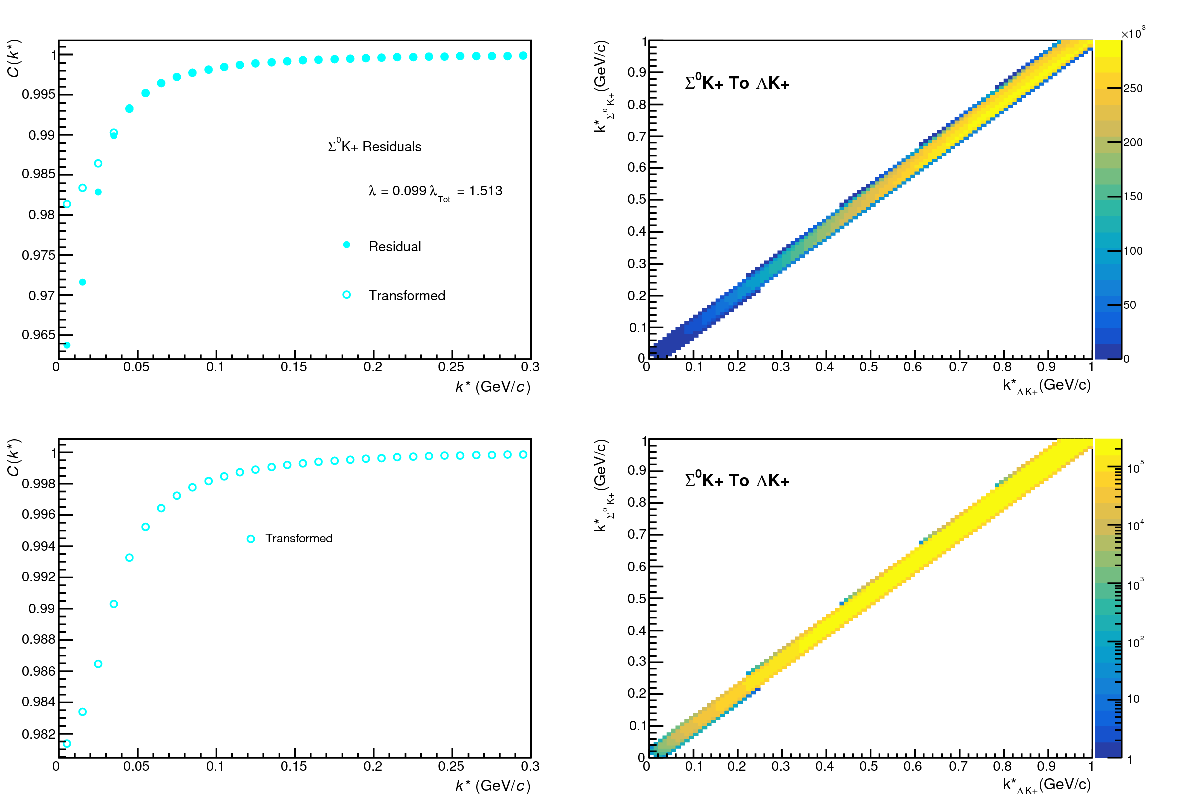
\includegraphics[width=\textwidth]{/home/jesse/Analysis/FemtoAnalysis/AnalysisNotes/5_Fitting/Figures/Residuals_LamKchP_0010_Sig0KchP_MomResCrctn_NonFlatBgdCrctn_10Res_PrimMaxDecay4fm_UsingXiDataAndCoulombOnly.pdf}
  \caption[$\Sigma^{0}$K$^{+}$ Transform]{$\Sigma^{0}$K$^{+}$ Transform.  These figures were taken using parameter values obtained from fits to the data.  In the top left corner of the figures, the input correlation function (closed symbols) is shown together with the output, transformed, correlation function (open symbols).  In the bottom left, the transformed correlation is shown by itself.  The right two plots in each figure show the transform matrix without (top right) and with (bottom right) a log-scale on the z-axis.}
  \label{fig:Sig0KchPtoLamKchPTransform}
\end{figure}


\begin{figure}[h]
  \centering
  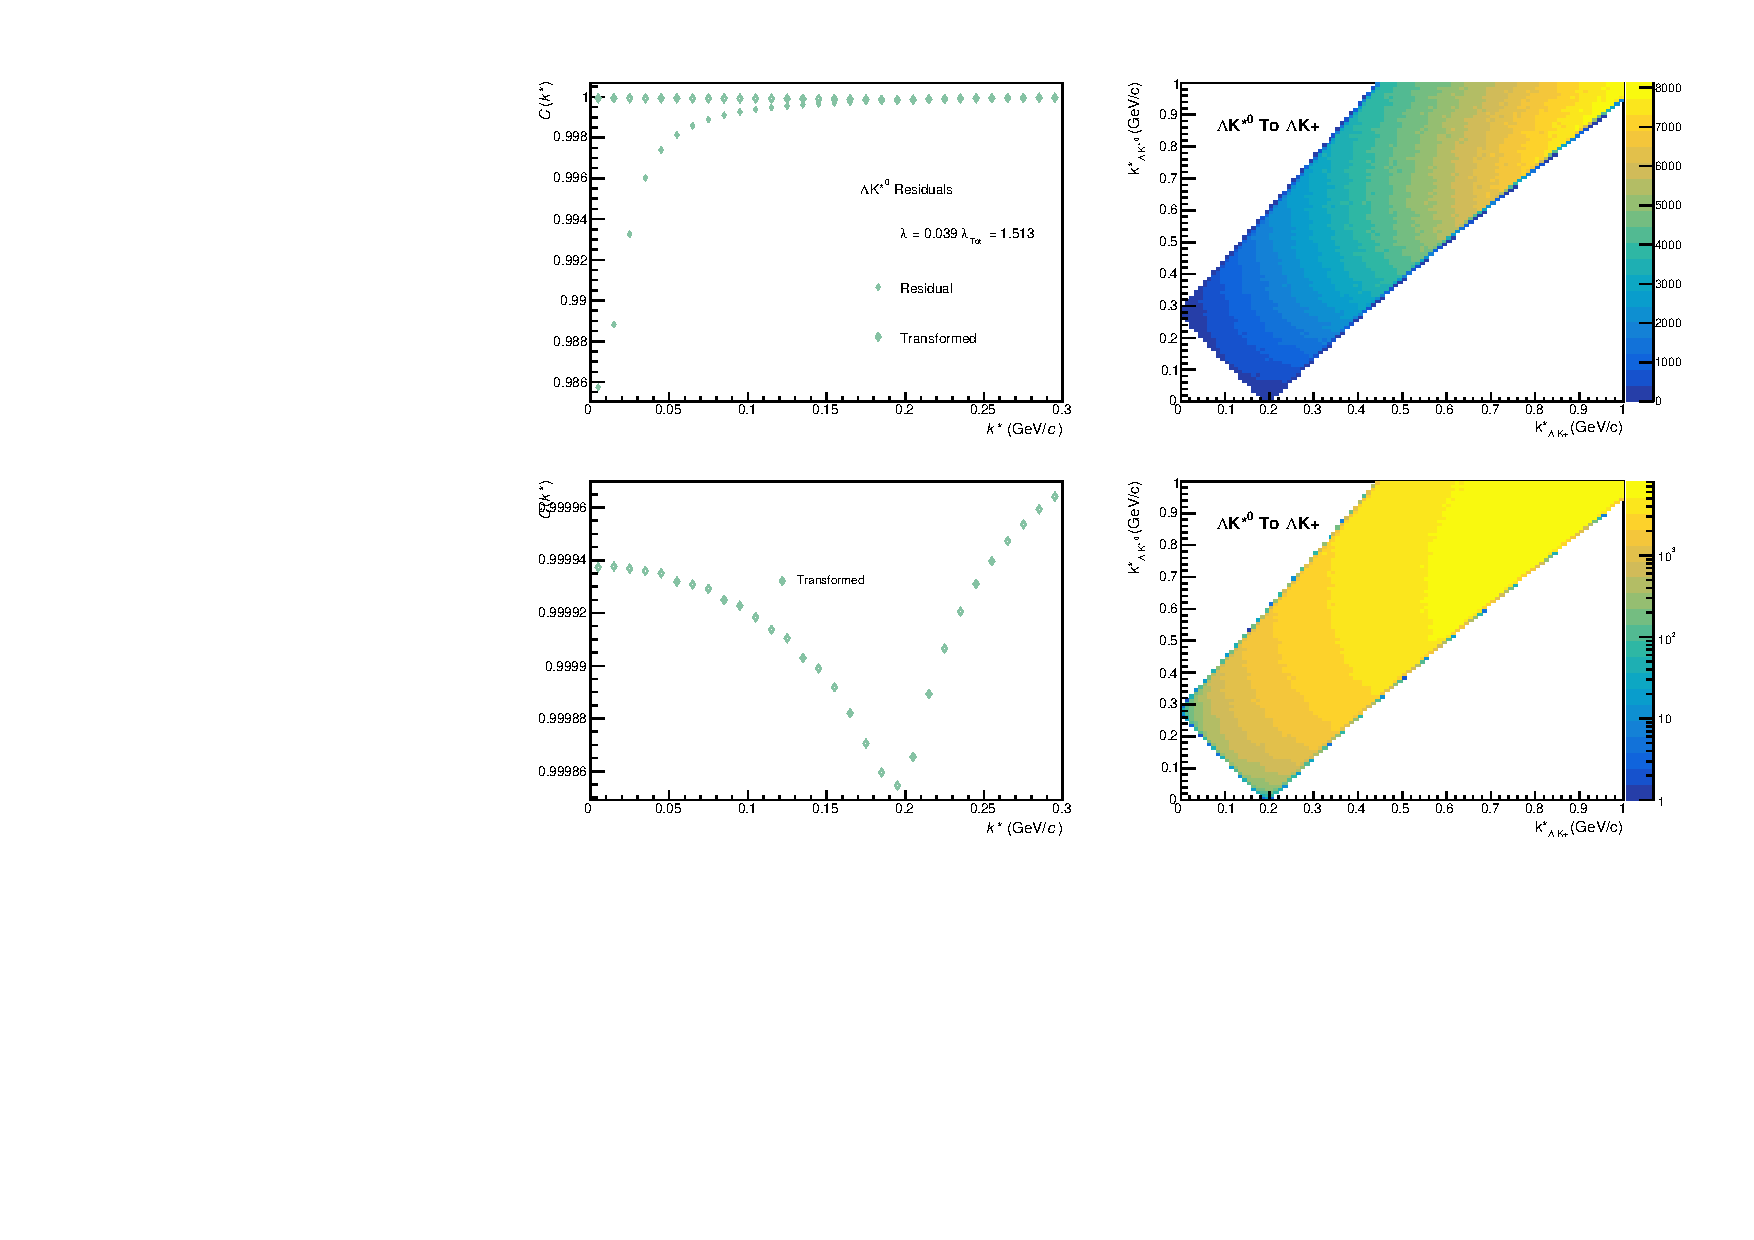
\includegraphics[width=\textwidth]{/home/jesse/Analysis/FemtoAnalysis/AnalysisNotes/5_Fitting/Figures/Residuals_LamKchP_0010_LamKSt0_MomResCrctn_NonFlatBgdCrctn_10Res_PrimMaxDecay4fm_UsingXiDataAndCoulombOnly.pdf}
  \caption[$\Lambda\mathrm{K^{*0}}$ Transform]{$\Lambda\mathrm{K^{*0}}$ Transform.  These figures were taken using parameter values obtained from fits to the data.  In the top left corner of the figures, the input correlation function (closed symbols) is shown together with the output, transformed, correlation function (open symbols).  In the bottom left, the transformed correlation is shown by itself.  The right two plots in each figure show the transform matrix without (top right) and with (bottom right) a log-scale on the z-axis.}
  \label{fig:LamKSt0toLamKchPTransform}
\end{figure}



Concerning the radii of the residual parent pairs, it was suggested that these should be set to smaller values than those of the daughter pair.  In the interest of minimizing the number of parameters in the fitter, we tested this by introducing an \mt-scaling of the parents' radii.  The motivation for this scaling comes from the approximate \mt-scaling of the radii observed in \ref{fig:mTScalingOfRadii_3Res}.  To achieve this scaling, we assume the radii follow an inverse-square-root distribution: $R_{AB} = \alpha m_{\mathrm{T}}^{-1/2}$.  Then, it follows that we should scale the parent radii as:

\begin{equation}
R_{AB} = R_{\Lambda K}\left(\frac{m_{\mathrm{T},AB}}{m_{\mathrm{T},\Lambda K}}\right)^{-1/2}
\label{eqn:mtscaling}
\end{equation}

The values of \mt for each pair system were taken from THERMINATOR.  As the fitter dances around parameter space and selects a new radius for the \LamK system, the radii of the residuals is simply the \LamK radius scaled by the appropriate factor, given above (Eq.\ref{eqn:mtscaling}).  In the end, this scaling factor made no significant difference in our fit results, so this complication is excluded from our final results.  Note that this is not surprising, as the most extreme scaling factor was, in the case of using 10 residual systems, between $\Lambda$K+ with $m_{\mathrm{T},\Lambda K+} \approx$ 1.4 GeV/$c^{2}$ and $\Xi^{-}$K$^{*0}$ with $m_{\mathrm{T},\Xi^{-} K^{*0}} \approx$ 1.8 GeV/$c^{2}$, resulting in a scale factor of $\approx$ 0.9.

\clearpage

\end{document}